\documentclass[a4paper, fleqn]{article}

\usepackage{import}
\import{.}{head}

\title{On Eberhard-type theorems.}
\author{Sebastian Manecke}
\makeindex
\begin{document}
\newcolumntype{M}{>{\centering\arraybackslash}m{\dimexpr.1\linewidth-2\tabcolsep}}
\newcolumntype{L}[1]{>{\raggedleft\arraybackslash}p{#1}}
\newcolumntype{R}[1]{>{\raggedright\arraybackslash}p{#1}}

\thispagestyle{empty}
\begin{titlepage}
\begin{center}


  \begin{tabular}{R{6.9cm} M p{6.9cm}}
    %  \begin{tabular}{rrM l}
    {\Large Technische Universität Dresden}&  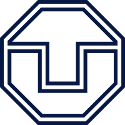
\includegraphics[scale =0.25]{TU.png} & \Large{Fachrichtung Mathematik}     
  \end{tabular}
  %{\Large Technische Universität Dresden\  {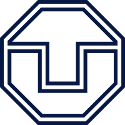
\includegraphics[scale = 0.25]{TU.png}} \ Fachrichtung Mathematik}

  \vfil

  {\Huge\ On Eberhard-like theorems}
  \\[\bigskipamount]
  \vfil
      {\LARGE
        Bachelorarbeit
        \\[\bigskipamount]
        zur Erlangung des ersten Hochschulgrades
        \\[\bigskipamount]
        Bachelor of Science  (B.Sc.)
        \\[\bigskipamount]
      }


      %\includegraphics[scale= 0.4]{title.png}


      vorgelegt von
      \\[\bigskipamount]
      Sebastian Manecke
      \\[\bigskipamount]
      (geboren am 29.4.1993 in Leipzig)
      \\[\bigskipamount]
      Tag der Einreichung: 6.3.2015
      \\[\bigskipamount]
      Prof. Ulrich Brehm, Institut für Geometrie
\end{center}
\end{titlepage}


\tableofcontents
\newpage
The thesis considers problems regarding the existence of polyhedra where for each $k \in \nats$ the number of $k$-gons in the polyhedron is given. The sequence of these numbers will be called the $p$-vector of the polyhedron. A basic question one could for example ask is ``Does there exist a polyhedron with exactly twelve pentagons and a hexagon?'' After several tries of building a solid with these conditions, one may come to the conclusion that no such polyhedron exists, and rightly so! From this assertion, further investigation could be done to search for a deeper reason for the existence or non-existence of a polyhedron for a given $p$-vector. One could try to find an exact criterion on the $p$-vector for realizability, but this seems to be a hard and out of scope problem. Viewing the problem from another angle is possible by using a combinatorical theorem known as ``Euler's relation''. This relation at first give no information about distinctive face counts for different number of sides, but by fixing some regularity of the realization and using several easy geometric properties of polygons one is able to transform ``Euler's relation'' to an interesting equation. The equation seems to imply that each face type has an inherent curvature which applies to the polyhedron. So for example triangles have a positive curvature and ``close'' the polyhedron, while heptagons and larger $k$-gons have negative curvature and seem to ``widen'' the realization. This equation only gives a necessary condition for realizability of the polyhedron, so there are nonetheless $p$-vectors satisfying this equation, but for which no realization exists. In view of this, the equation admits the possibility to add in some more polygons which act flat - they give in sum no positive or negative curvature. So while some sequences are not realizable, maybe it is possible to add some more polygons with no total curvature and try realize this sequence. A theorem which states that this is always possible (where the exact meaning of ``this'' will be defined later) will be called a general Eberhard's theorem. This thesis proves some of these theorems positively and also gives some examples where adding certain polygons does not help in the realization. The structure of this thesis is as following: The first two sections specify the conditions and equations stated above and introduce notation and the arguments used. The next five sections are devoted to a general Eberhard's theorem and prove them fully where possible. The last two sections give conditions where one can not hope for a general Eberhard's theorem and insight to some extensions to the present work. Each proof uses one or more figures to describe a construction. The general reading on most of them is ``the image shown left is transformed to the one on the right'' if the image is about to describe a specific transformation.

\section{Preliminaries}

% Todo: define $p$-vector, $f$-vector, $v$-vector
% realization of a $p$-vector, notation of a $p$-vector, independence of length
\begin{definition}[Sequence]
  A sequence $a$ in this thesis is a map $\nats \setminus \{0, 1, 2\} \rightarrow \nats$ with finite support. These maps will be written as $(a(3), a(4), ..., a(k))$, where $k = \operatorname{max} \operatorname{supp} a$. If $a$ has a small but wide support these notation will be further abbreviated as $[a(k_1) \times k_1, a(k_2) \times k_2, ...]$, where $a(k) \times k$ will be simply written as $k$ if $a(k) = 1$.
\end{definition}
\begin{example}
  $(2, 0, 0, 1)$, $[2 \times 3, 1 \times 6]$ and $[2 \times 3, 6]$ all denote the same sequence. 
\end{example}
\begin{definition}[$p$-vector and $v$-vector of an polyhedron]\label{def:relizable}
  The $p$-vector of a polyhedron $P$ is the sequence $(p_3, \dots, p_m)$, where $p_k$ denotes the number of faces with exactly $k$ vertices. Similarily the $v$-vector of $P$ is the sequence $(v_1, \dots, v_n)$, where each $v_k$ measures the number of edges of $P$ with valence $k$. 
\end{definition}

\begin{definition}
Sequences $a = (a_3, \dots, a_m)$, $b = (b_3, \dots, b_m)$ are said to be realizable, if there exists a polyhedron which has $a$ is its $p$-vector and $b$ as its $v$-vector.
\end{definition}

With this setup, we want to discuss in this thesis a broad problem arising from the combinatorical properties of polyhedra:
\begin{problem} Are two arbitrarily given sequences realizable?
\end{problem}
The most basic result answering that question partially is Eulers relation.
\begin{theorem}[Eulers relation]\label{thm:eulers:relation}
  For each polyhedron with $v$ vertices, $e$ edges and $f$ faces
  \begin{align*}
    v - e + f = 2
  \end{align*}
  holds.
\end{theorem}
Given the notation as above one can immediatly draw some basic conclusions from this relation: For one the number of vertices $v$ is obviously the sum of the entries of $v$-vector, as is the same with $f$, which is the sum of the $p$-vector. Using a double counting argument (each edge is adjacent to two faces and each edge is adjacent to two vertices) the following for the number of edges holds:
\begin{align*}
  2e = \sum_{k=3}^{m} k \cdot p_k = \sum_{k=3}^{n} k \cdot f_k
\end{align*}
Putting these equations in Eulers relation \autoref{thm:eulers:relation} gives for some $t \in (0, 1)$
\begin{align*}
  \sum_{k=3}^m v_k - \left(\frac{t}{2} \sum_{k=3}^m k v_k + \frac{1-t}{2} \sum_{k=3}^n k p_k \right) + \sum_{k=3}^n p_k = 2
\end{align*}
which can be transformed into:
\begin{align*}
  t \sum_{k=3}^m \left(\frac{2}{t} - k \right) v_k + (1-t) \sum_{k=3}^n \left( \frac{2}{1-t} - k \right) p_k = 4.
\end{align*}
This equation can be independant of the value of some $v_k$ or $p_{k'}$ when the value of $t$ is appropriately choesen. Of special interest in this thesis are the cases of one $v_r$ giving no information in the above equation (so $r \geq 3$ fixed and $t = \frac{2}{r}$) and having $v_{k} = 0$ for each $k \geq 3$, $k \neq r$. The resulting polyhedron has the property that each of his vertices has valence $r$. 
% TODO Explain this.
\begin{definition}[$r$-realizable]
  A sequence $a = (a_3, \dots, a_m)$ is said to be $r$-realizable, if there exists a polyhedron such that $a$ is realizable with an $v$-vector consisting only of valence $r$ (in the sense of \autoref{def:relizable}).
\end{definition}
Under these circumstances $r$ has to be in $\{3, 4, 5\}$.

For $r \in \{3, 4, 5\}$ the following equations arise:
\begin{align}
  r &= 3: \sum_{k=3}^n \left(6 - k \right) p_k = 12 \label{eq:valence:3}\\
  r &= 4: \sum_{k=3}^n \left(4 - k \right) p_k = 8  \label{eq:valence:4}\\
  r &= 5: \sum_{k=3}^n \left( \frac{10}{3} - k \right) p_k = \frac{20}{3} \label{eq:valence:5}\\
\end{align}
\begin{notation}
  If an $p$-vector $(p_3, \dots, p_k)$ is meant to be seen in this context, that each vertex of the considered polyhedron has valence $r$, this valence will be appended to the sequance, i.e. $(p_3, \dots, p_k)_r$.
\end{notation}
Even in with this rather specific constraints the problem stated above has no easy definite answer, as in, not every $p$-vector satisfying on of these equations can be realized as an polyhedron.
\begin{example}
  The $p$-vector $(0, 12, 1)_3$ has no realization but satisfies \autoref{eq:valence:3}. To see this one can start with one hexagon. As only pentagons are left to build the rest of the polyhedron a ring of six pentagons has to be glued to the hexagon. Another ring of six pentagons is forced to be glued to the first leaving a hole of the shape of an hexagon in the end, but no polygons left to fill it.

  \begin{tikzfigure}{\label{fig:preliminaries:example}}
\begin{scope}[xscale=1.0, yscale=0.866]
          \draw (-1, 0) -- ++(0.5, -1) -- ++(1, 0) -- ++(0.5, 1) -- ++(-0.5, 1) -- ++(-1, 0) -- ++(-0.5, -1);
          \draw (-1, 0) -- (-2, 0) -- (-2.25, -1.5) -- (-1, -2) -- (-0.5, -1);
          \draw (1, 0) -- (2, 0) -- (2.25, -1.5) -- (1, -2) -- (0.5, -1);
          \draw (-0.5, 1) -- (-1, 2) -- (0, 3) -- (1, 2) -- (0.5, 1);
          \draw (-1, -2) -- (0, -3) -- (1, -2);
          \draw (-2, 0) -- (-2.25, 1.5) -- (-1, 2);
          \draw (2, 0) -- (2.25, 1.5) -- (1, 2);
          \draw (-3, -2) -- (-3, 2) -- (0, 4) -- (3, 2) -- (3, -2) -- (0, -4) -- (-3, -2);
          \draw (-3, -2) -- (-2.25, -1.5);
          \draw (3, -2) -- (2.25, -1.5);
          \draw (-3, 2) -- (-2.25, 1.5);
          \draw (3, 2) -- (2.25, 1.5);
          \draw (0, -4) -- (0, -3);
          \draw (0, 4) -- (0, 3);
        \end{scope}   
    
  \end{tikzfigure}
  
\end{example}

\begin{problem}[General Eberhard's problem]
  Let $r \in \{3, 4, 5\}$ and $(q_3, \dots)$ be a sequence which satisfies 
  \begin{align}
    r &= 3: \sum_{k=3}^n \left( 6            - k \right) q_k = 0 \label{eq:zero:curv:3}\\
    r &= 4: \sum_{k=3}^n \left( 4            - k \right) q_k = 0 \label{eq:zero:curv:4}\\
    r &= 5: \sum_{k=3}^n \left( \frac{10}{3} - k \right) q_k = 0 \label{eq:zero:curv:5}
  \end{align}
  in the respective cases. Then show that for all sequences $(p_3, \dots)$  satisfying the respective \autoref{eq:valence:3}, \autoref{eq:valence:4} or \autoref{eq:valence:5}, there exists an $c \in \nats$ for which $(p_3 + c \cdot q_3, p_4 + c \cdot q_4, \dots)$ is realizable as a polyhedron.
\end{problem}
\begin{notation}
  Throughout the thesis we want to denote this problem as of $(p_3, \dots, p_n)_r$-type.
\end{notation}
\begin{definition}[$r$-realizable]
  A sequence $a = (p_3, \dots, p_m)$ is said to be $(q_3, \dots, q_n)_r$-realizable, if there exists a polyhedron such that $a$ is realizable with an $v$-vector consisting only of valence $r$ (in the sense of \autoref{def:relizable}).
\end{definition}

\autoref{eq:valence:3} and \autoref{eq:valence:4} suggest that $(6)_3$ or $(4)_4$ might be good candidates for such statements. As it is, these questions are both proved and are known as the (non-general) Eberhards theorem in \cite{ConvexPolytopes}:
\renewcommand{\Itemautorefname}{Theorem \ref{thm:eberhard}}
\begin{theorem}[Eberhards theorem] \label{thm:eberhard} The following holds:
  \begin{enumerate}[label=(\roman*)]
  \item \label{thm:eberhard:3} For each $p_3, p_4, p_5, p_7, \dots, p_m$ satisfiying \autoref{eq:valence:3} there exists a number $p_6$ such that $(p_3, \dots, p_m)$ is realizable. 
  \item \label{thm:eberhard:4} For each $p_3, p_5, \dots, p_m$ satisfiying \autoref{eq:valence:4} there exists a number $p_4$ such that $(p_3, \dots, p_m)$ is realizable. 
  \end{enumerate}
\end{theorem}

A stronger theorem, which generalizes the first case, is given in \cite{jendrol1977generalization}.

Building upon these two, this thesis will present a bunch of new theorems of general Eberhards type. One of these proofs takes a similar approach as the proof given in \cite{ConvexPolytopes} for \autoref{thm:eberhard:4}. The rest of the proofs directly use \autoref{thm:eberhard}. This is done by taking a sequence not too different form the given one which suffices either \autoref{eq:valence:3} or \autoref{eq:valence:4}, constructing a polyhedron by the statements of \autoref{thm:eberhard} and then by adding or deleting some polygons to create a polyhedron with a $p$-vector as stated. This is done by either substituting edges and vertices or every face by some larger structure. 


%Todo Steinars theorem.
\newpage
\section{Arcs}

Let $r \in \nats$. For the rest of this section one can think of $r$ as the given valence of a polyhedron. Many constructions in this thesis will utilize the concept of replacing each face of a polyhedron with a larger structure. It can be quite challenging to see whether the resulting structures fit together as the previous faces did. This chapter introduces the necessary formalism for these kind of constructions.

\begin{definition}[Arc]
  An arc with weights $w_1, \dots, w_n$ is cycle (in the sense of graph theory) of length $n$ with vertices of weight $w_1, \dots, w_n \in \{0, \dots, r - 2\}$ where the vertices of each pair of weights $w_i, w_{i+1}$ are neighboring. An $n$-gon with the weights $r-1$ on each vertex is called $n$-arc. A piece of an arc with weights $w_1, \dots, w_n$ is a path of length $n$, where each vertex is weighted with $w_1, \dots w_n$ and $w_i, w_{i+1}$ denote weights of neighboring vertices. These weights will also be called the face count of the vertex. 
\end{definition}

This definition has of cause a geometric interpretation. For a given graph, where each vertex has valence at most $r$ a fixed cycle in this graph can be interpreted as an arc where each vertex $v$ is given the weight $\deg (v) - 1$, where $\deg (v)$ denotes the degree of the vertex $v$, thus, as the definition suggests, each weight counts the number of faces adjacent to $v$. To quickly describe pieces of an arc his weight will be inscribed in connected circles, like  \piece{1}--\piece{2}--\piece{1}--\piece{2} for a piece of an arc of length $4$ with weights $1, 2, 1$ and $2$.
\begin{definition}
  A planar graph is called a $r$-component if every of its vertices except the ones on the outer face is $r$-valent (the exterior vertices can differ from the valence $r$, but are not required to). The outer face can be interpreted as an arc, where each vertex $v$ the weight $\deg(v) - 1$ is given. This arc will be called the outer arc.
\end{definition}

If one is interested in whether to parts of a construction fit together to assemble a larger part one has to compare the valences along some path on the boundary of each part. This is captured in the following definition:
\begin{definition}
  Two pieces of an arc with weights $w_1, \dots, w_{n}$ and $w'_1, \dots, w'_{n}$ are said to fit together if for all $i \in \{1, \dots, n \}$ holds $w_i + w'_{n-i} = r$. A piece of an arc is called self-fitting if it fits with itself.
\end{definition}

\begin{lemma}\label{thm:fitting:arcs}
  Let $G, G'$ be two $r$-components. Fix an orientation on both of them (clockwise or counter-clockwise) and let $v_0, \dots, v_{n+1}$ and $v'_0, \dots, v'_{n+1}$ be consecutive vertices (under this orientation) on $G, G'$ with weights $w_0, \dots, w_{n+1}$ and $w'_0, \dots, w'_{n+1}$. If $w_0 + w'_{n+1} + 1 \leq r$ and $w'_0 + w_{n+1} + 1 \leq r$ and the pieces $v_1, \dots, v_n$ and $v'_1, \dots, v'_n$ fit together, then there exists a $r$-component which has $G$ and $G'$ as subgraphs which identifies $v_0 = v'_{n+1}, \dots v_{n+1} = v'_0$, but not any other two vertices.
  \begin{proof}
    By ``gluing'' $G$ and $G'$ along the paths $v_0 - \dots - v_{n+1}$ and $v'_0 - \dots - v'_{n+1}$, the resulting graph fulfills the requirements. It is planar since both $G$ and $G'$ are and both graphs where combined along the outer arc. Let $\tilde{v}_i$ be vertex in the new graph which represents $v_i$ and $v_{n+1-i}$ from the old graphs. When gluing $v_i$ with $v_{n+1-i}$ ($1 \leq i \leq n$), the edges $v_{i-1}$--$v_i$ and $v'_{n + 1 - i}$--$v'_{n + 2 - i}$ coincide, as well as the edges $v'_{n - i}$--$v'_{n + 1 - i}$ and $v_i$--$v_{i+1}$. Therefore the valence of $\tilde{v}_i$ is two less then the sum of valences of $v_i$ and $v'_{n+1-i}$, thus
    \begin{equation*}
      \deg(\tilde{v}_i) = \deg(v_i) + \deg(v'_{n+1-i}) - 2 = w_i + 1 + w'_{n + 1 - i} + 1 - 2 = w_i + w'_{n + 1 - i} = r.
    \end{equation*}
    The edges $v_0$--$v_1$ and $v'_n$--$v'_{n+1}$ are now glued together, it follows $\deg(\tilde{v}_0) = \deg(v_0) + \deg(v'_{n+1}) - 1 = (w_0 + 1) + (w'_{n+1} + 1) - 1 = w_0 - w'_{n+1}) + 1 \leq r$. This proves that the new graph is a $r$-component.
  \end{proof}
\end{lemma}

TODO: Insert picture for demonstration purposes.

\begin{definition}
  Let $p$ be a piece of an arc with weights $w_1, \dots, w_{n}$. The $p$-expansion of an arc $a$ with weights $a_1, \dots a_k$ is the arc with weights $a_1, w_1, \dots w_n, a_2, w_1, \dots, w_n, a_3 \dots, a_k, w_1, \dots, w_n$.
\end{definition}

With this, one is able to describe a general construction scheme:

\begin{construction}\label{thm:construction:arcs} Let $G$ be a planar graph of valence $r$. Let $p$ be a self-fitting piece of an arc. During the construction each $n$-gonal face is replaced with a $r$-component, whose outer arc is the $p$-expansion of a $n$-arc. This construction leads to a connected planar graph of valence $r$.
  \begin{proof}
    When viewing each face as a $r$-component, \autoref{thm:fitting:arcs} ensures that the valences of the new vertices inserted between the original vertices of one face sum up with the valences of the respective vertices added to a previously adjacent face to the required valence of $r$. TODO.
  \end{proof}
\end{construction}

\begin{remark}
  \autoref{thm:construction:arcs} still holds on an orientable closed $2$-manifold, as the arguments used were only ``local planarity'' and the existence of an orientation, thus \autoref{thm:fitting:arcs} can be used for all pairs of adjacent faces. If the piece of an arc of length $n$ is also symmetric, that is, $w_i = w_{n-i}$, $i = 1, \dots n$, even the requirement of an orientation can be dropped, the necessary equations of \autoref{thm:fitting:arcs} then hold regardless of the numbering of the vertices. If $w_i$ is a weight in a symmetric self-fitting piece of an arc of length $n$, then $w_i + w_{n-i} = 2 w_i = r$, therefore for these kinds of arcs to exists $r$ has to be even; reviewing the considered cases only $r = 4$ remains.
\end{remark}
\newpage
\section{The case $[5, 7]_3$}
\begin{theorem}
    Let $p = (p_3, p_4, p_5, \dots, p_n)$ be a given sequence satisfying equation \ref{eq_valence_3}, then there exists $r \in \nats$ for which $p + r [5, 7]_3$ is $3$-realizable.
    \begin{proof}
      \heartpar{
  The proof starts by using the construction given by Eberhards Theorem \ref{thm_eberhard}(\ref{thm_eberhard_3}). This results in a realization of $p$ which has many more hexagons then needed. The next step is to remove these hexagons and replace them by pentagons and heptagons. To further proceed, one adds a ring of hexagons around each polygon in the realization, these will be replaced immediately but serve the purpose of adding space around each polygon which can be used for replacement with pentagons and heptagons. The process is illustrated below:
}
  \begin{figure}[htpp]
    \centering
    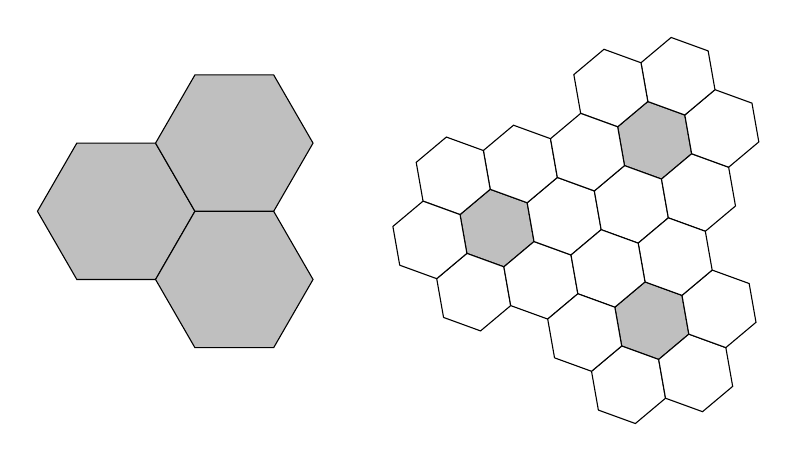
\begin{tikzpicture}
      \matrix (m) [ column sep=1cm] {
          \begin{scope}[xscale=1.0, yscale=0.866]
            \filldraw[fill=gray!50!white] (0, 1) -- ++(0.5, -1) -- ++(1, 0) -- ++(0.5, 1) -- ++(-0.5, 1) -- ++(-1, 0) -- ++(-0.5, -1);
            \filldraw[fill=gray!50!white] (1.5, 0) -- ++(0.5, -1) -- ++(1, 0) -- ++(0.5, 1) -- ++(-0.5, 1) -- ++(-1, 0) -- ++(-0.5, -1);
            \filldraw[fill=gray!50!white] (1.5, 2) -- ++(0.5, -1) -- ++(1, 0) -- ++(0.5, 1) -- ++(-0.5, 1) -- ++(-1, 0) -- ++(-0.5, -1);
          \end{scope}
        &


          \begin{scope}[rotate=40, xscale=1.0, yscale=0.866, scale=0.5] 
            \filldraw[fill=gray!50!white] (0, 1) -- ++(0.5, -1) -- ++(1, 0) -- ++(0.5, 1) -- ++(-0.5, 1) -- ++(-1, 0) -- ++(-0.5, -1);
            \filldraw[fill=white] (-1.5, 0) -- ++(0.5, -1) -- ++(1, 0) -- ++(0.5, 1) -- ++(-0.5, 1) -- ++(-1, 0) -- ++(-0.5, -1);
          \filldraw[fill=white] (0, -1) -- ++(0.5, -1) -- ++(1, 0) -- ++(0.5, 1) -- ++(-0.5, 1) -- ++(-1, 0) -- ++(-0.5, -1);
          \filldraw[fill=white] (1.5, 0) -- ++(0.5, -1) -- ++(1, 0) -- ++(0.5, 1) -- ++(-0.5, 1) -- ++(-1, 0) -- ++(-0.5, -1);
          \filldraw[fill=white] (1.5, 2) -- ++(0.5, -1) -- ++(1, 0) -- ++(0.5, 1) -- ++(-0.5, 1) -- ++(-1, 0) -- ++(-0.5, -1);
          \filldraw[fill=white] (0, 3) -- ++(0.5, -1) -- ++(1, 0) -- ++(0.5, 1) -- ++(-0.5, 1) -- ++(-1, 0) -- ++(-0.5, -1);
          \filldraw[fill=white] (-1.5, 2) -- ++(0.5, -1) -- ++(1, 0) -- ++(0.5, 1) -- ++(-0.5, 1) -- ++(-1, 0) -- ++(-0.5, -1);

          \filldraw[fill=gray!50!white] (4.5, 0) -- ++(0.5, -1) -- ++(1, 0) -- ++(0.5, 1) -- ++(-0.5, 1) -- ++(-1, 0) -- ++(-0.5, -1);
          \filldraw[fill=white] (3, -1) -- ++(0.5, -1) -- ++(1, 0) -- ++(0.5, 1) -- ++(-0.5, 1) -- ++(-1, 0) -- ++(-0.5, -1);
          \filldraw[fill=white] (4.5, -2) -- ++(0.5, -1) -- ++(1, 0) -- ++(0.5, 1) -- ++(-0.5, 1) -- ++(-1, 0) -- ++(-0.5, -1);
          \filldraw[fill=white] (6, -1) -- ++(0.5, -1) -- ++(1, 0) -- ++(0.5, 1) -- ++(-0.5, 1) -- ++(-1, 0) -- ++(-0.5, -1);
          \filldraw[fill=white] (6, 1) -- ++(0.5, -1) -- ++(1, 0) -- ++(0.5, 1) -- ++(-0.5, 1) -- ++(-1, 0) -- ++(-0.5, -1);
          \filldraw[fill=white] (4.5, 2) -- ++(0.5, -1) -- ++(1, 0) -- ++(0.5, 1) -- ++(-0.5, 1) -- ++(-1, 0) -- ++(-0.5, -1);
          \filldraw[fill=white] (3, 1) -- ++(0.5, -1) -- ++(1, 0) -- ++(0.5, 1) -- ++(-0.5, 1) -- ++(-1, 0) -- ++(-0.5, -1);
          
          \filldraw[fill=gray!50!white] (1.5, -4) -- ++(0.5, -1) -- ++(1, 0) -- ++(0.5, 1) -- ++(-0.5, 1) -- ++(-1, 0) -- ++(-0.5, -1);
          \filldraw[fill=white] (0, -5) -- ++(0.5, -1) -- ++(1, 0) -- ++(0.5, 1) -- ++(-0.5, 1) -- ++(-1, 0) -- ++(-0.5, -1);
          \filldraw[fill=white] (1.5, -6) -- ++(0.5, -1) -- ++(1, 0) -- ++(0.5, 1) -- ++(-0.5, 1) -- ++(-1, 0) -- ++(-0.5, -1);
          \filldraw[fill=white] (3, -5) -- ++(0.5, -1) -- ++(1, 0) -- ++(0.5, 1) -- ++(-0.5, 1) -- ++(-1, 0) -- ++(-0.5, -1);
          \filldraw[fill=white] (3, -3) -- ++(0.5, -1) -- ++(1, 0) -- ++(0.5, 1) -- ++(-0.5, 1) -- ++(-1, 0) -- ++(-0.5, -1);
          \filldraw[fill=white] (1.5, -2) -- ++(0.5, -1) -- ++(1, 0) -- ++(0.5, 1) -- ++(-0.5, 1) -- ++(-1, 0) -- ++(-0.5, -1);
          \filldraw[fill=white] (0, -3) -- ++(0.5, -1) -- ++(1, 0) -- ++(0.5, 1) -- ++(-0.5, 1) -- ++(-1, 0) -- ++(-0.5, -1);
        \end{scope};
        \\
      };
  \end{tikzpicture}
  \end{figure}


  One now chooses a set $S$ of hexagons one wants to keep, $|S| = p_6$. Each hexagon not in $S$ and the surrounding six hexagons are replaced by the following structure: 

  \begin{figure}[htpp]
    \centering
    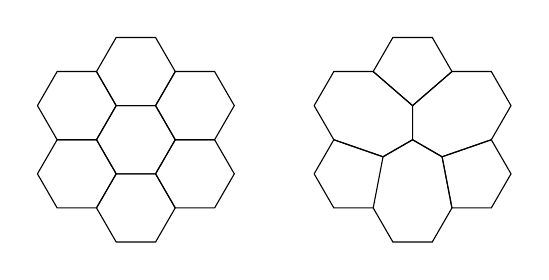
\begin{tikzpicture}
      \matrix (m) [ column sep=1cm] {
        \begin{scope}[xscale=1.0, yscale=0.866, scale=0.5]
          \draw (0, 1) -- ++(0.5, -1) -- ++(1, 0) -- ++(0.5, 1) -- ++(-0.5, 1) -- ++(-1, 0) -- ++(-0.5, -1);
          \draw (-1.5, 0) -- ++(0.5, -1) -- ++(1, 0) -- ++(0.5, 1) -- ++(-0.5, 1) -- ++(-1, 0) -- ++(-0.5, -1);
          \draw (0, -1) -- ++(0.5, -1) -- ++(1, 0) -- ++(0.5, 1) -- ++(-0.5, 1) -- ++(-1, 0) -- ++(-0.5, -1);
          \draw (1.5, 0) -- ++(0.5, -1) -- ++(1, 0) -- ++(0.5, 1) -- ++(-0.5, 1) -- ++(-1, 0) -- ++(-0.5, -1);
          \draw (1.5, 2) -- ++(0.5, -1) -- ++(1, 0) -- ++(0.5, 1) -- ++(-0.5, 1) -- ++(-1, 0) -- ++(-0.5, -1);
          \draw (0, 3) -- ++(0.5, -1) -- ++(1, 0) -- ++(0.5, 1) -- ++(-0.5, 1) -- ++(-1, 0) -- ++(-0.5, -1);
          \draw (-1.5, 2) -- ++(0.5, -1) -- ++(1, 0) -- ++(0.5, 1) -- ++(-0.5, 1) -- ++(-1, 0) -- ++(-0.5, -1);
        \end{scope};

        &

        \begin{scope}[xscale=1.0, yscale=0.866, scale=0.5] 
          \draw (-1.5, 0) -- ++(0.5, -1) -- ++(1, 0) -- ++(0.25, 1.5) -- ++(-1.25, 0.5) -- ++(-0.5, -1);
          \draw (0, -1) -- ++(0.5, -1) -- ++(1, 0) -- ++(0.5, 1) -- ++(-0.25, 1.5) -- ++(-0.75, 0.5) -- ++(-0.75, -0.5);
          \draw (1.75, 0.5) -- ++(0.25, -1.5) -- ++(1, 0) -- ++(0.5, 1) -- ++(-0.5, 1) -- ++(-1.25, -0.5);
          \draw (1, 1) -- ++(0.75, -0.5) -- ++(1.25, 0.5) -- ++(0.5, 1) -- ++(-0.5, 1) -- ++(-1, 0) -- ++(-1, -1);
          \draw (0, 3) -- ++(1, -1) -- ++(1, 1) -- ++(-0.5, 1) -- ++(-1, 0) -- ++(-0.5, -1);
          \draw (-1.5, 2) -- ++(0.5, -1) -- ++(1.25, -0.5) -- ++(0.75, 0.5) -- ++(0, 1) -- ++(-1, 1) -- ++(-1, 0) -- ++(-0.5, -1);
        \end{scope};
        
        \\
      };
  \end{tikzpicture}
  \end{figure}

  For the remaining hexagons and all other kinds of polygons this ring structure is replaced differently, for each $n$-gon $n$ pentagons and $n$ heptagons replace the ring of hexagons:


    \begin{figure}[htpp]
    \centering
    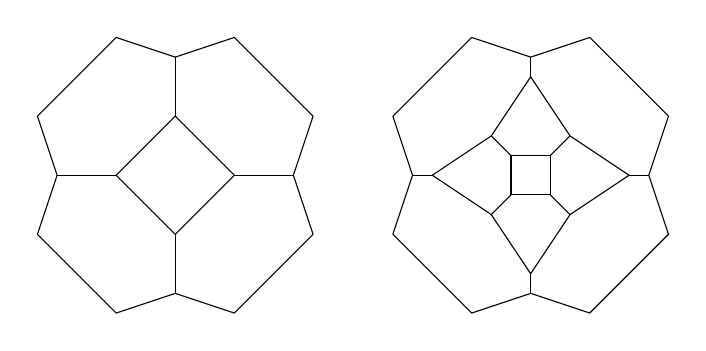
\begin{tikzpicture}
      \matrix (m) [ column sep=1cm] {

        \begin{scope}[scale=0.25] 
          \draw (-3, 0) -- (0, -3) -- (3, 0) -- (0, 3) -- (-3, 0);
          \draw (-3, 0) -- (-6, 0);
          \draw (0, -3) -- (0, -6);
          \draw (3, 0) -- (6, 0);
          \draw (0, 3) -- (0, 6);
          \draw (-6, 0) -- (-7, -3) -- (-3, -7) -- (0, -6) -- (3, -7) -- (7, -3) -- (6, 0) -- (7, 3) -- (3, 7) -- (0, 6) -- (-3, 7) -- (-7, 3) -- (-6, 0);
        \end{scope}
        &
        \begin{scope}[scale=0.25] 
          \draw (-6, 0) -- (-7, -3) -- (-3, -7) -- (0, -6) -- (3, -7) -- (7, -3) -- (6, 0) -- (7, 3) -- (3, 7) -- (0, 6) -- (-3, 7) -- (-7, 3) -- (-6, 0);
          \draw (-5, 0) -- (-6, 0);
          \draw (0, -5) -- (0, -6);
          \draw (5, 0) -- (6, 0);
          \draw (0, 5) -- (0, 6);

          \draw (-5, 0) -- (-2, -2) -- (0, -5) -- (2, -2) -- (5, 0) -- (2, 2) -- (0, 5) -- (-2, 2) -- (-5, 0);
          \draw (-2, -2) -- (-1, -1);
          \draw (2, -2) -- (1, -1);
          \draw (2, 2) -- (1, 1);
          \draw (-2, 2) -- (-1, 1);
          
          \draw (-1, -1) -- (1, -1) -- (1, 1) -- (-1, 1) -- (-1, -1);

        \end{scope}
        
        \\
      };
  \end{tikzpicture}
  \end{figure}
  This finishes the proof.
\end{proof}
\end{theorem}



\section{The case $[5, 8]_3$}
\begin{construction}\label{thm:construction:5:8}
  Given a $3$-valent polyhedron $P$ with $p$-vector $(p_3, p_4, p_5, p_6, p_7, p_8, \dots, p_m)$ and $p'_6 \leq p_6$, there exists another $3$-valent polyhedron $P'$ with $p$-vector $(p_3, p_4, p'_5, p'_6, p_7, p'_8, \dots, p_m)$, where $2(p'_5 - p_5) = p'_8 - p_8$.
  \begin{proof}
    As seen in \autoref{fig:case:5:8:img1}, one can create a (\piece{2}--\piece{1}--\piece{2}--\piece{1})-expansion of each polygon of the given realization $P$ (when counting the vertices clockwise). The construction forms around these $n$-gons a ring of pentagons, around which another ring of octagons is added. The resulting figure has $n$ vertices of valence $3$ on the outer arc, these will be the positions for final set of $n$ pentagons resulting in the shape given in \autoref{fig:case:5:8:img1}. It has the required outer arc since \piece{2}--\piece{1}--\piece{2}--\piece{1} is self-fitting, and therefore by \autoref{thm:construction:arcs} it gives rise to an polyhedron $\tilde{P}$.
    \begin{tikzfigure}{\label{fig:case:5:8:img1}}
      \matrix (m) [ column sep=1cm] {
        \begin{scope}
          \fill[fill=gray!50!white] (-1, -1) -- (1, -1) -- (1, 1) -- (-1, 1);
          \draw (-1, -1) circle[radius=2pt] -- (1, -1) circle[radius=2pt] -- (1, 1) circle[radius=2pt] -- (-1, 1) circle[radius=2pt] -- (-1, -1);
        \end{scope}
        &
        \begin{scope}[scale=0.25] 
          \draw (-6, 0) -- (-7, -3) -- (-6, -6) -- (-3, -7) -- (0, -6) -- (3, -7) -- (6, -6) -- (7, -3) -- (6, 0) -- (7, 3) -- (6, 6) -- (3, 7) -- (0, 6) -- (-3, 7) -- (-6, 6) -- (-7, 3) -- (-6, 0);
          \draw (-5, 0) -- (-6, 0);
          \draw (0, -5) -- (0, -6);
          \draw (5, 0) -- (6, 0);
          \draw (0, 5) -- (0, 6);

          \draw (-5, 0) -- (-2, -2) -- (0, -5) -- (2, -2) -- (5, 0) -- (2, 2) -- (0, 5) -- (-2, 2) -- (-5, 0);
          \draw (-2, -2) -- (-1, -1);
          \draw (2, -2) -- (1, -1);
          \draw (2, 2) -- (1, 1);
          \draw (-2, 2) -- (-1, 1);
          
          \filldraw[fill=gray!50!white] (-1, -1) -- (1, -1) -- (1, 1) -- (-1, 1) -- (-1, -1);
          \draw (-7, -3)  -- (-9, -1) -- (-9, 1) circle[radius=8pt]-- (-7, 3);
          \draw ( 7, -3) -- ( 9, -1) circle[radius=8pt]-- ( 9, 1) -- ( 7, 3) ;
          \draw (-3, -7) -- (-1, -9) circle[radius=8pt]-- (1, -9) -- (3, -7) ;
          \draw (3, 7) -- (1, 9) circle[radius=8pt]-- (-1, 9) -- (-3, 7);

        \end{scope}
        \\
      };
    \end{tikzfigure}

    In view of the hexagons one can now replace the figure held in the first construction step with the ones seen in \autoref{fig:case:5:8:img2}. Note that the left side of the figure is the result of the above construction in the case of an hexagon and the right side has the same outer arc, but consists only of pentagons and octagons. So one can substitute arbitrarly many hexagons by an amount of octagons and heptagons, creating hereby $P'$. $2(p'_5 - p_5) = p'_8 - p_8$ holds, since \autoref{eq:valence:3} holds for $P$ as well as for $P'$.
    
    \begin{tikzfigure}{\label{fig:case:5:8:img2}}
      \matrix (m) [ column sep=1cm] {

        \begin{scope}[rotate=-30, yscale=0.866, scale=0.25] 
          \draw (-1, 8) -- (1, 8) -- (1.5, 7) -- (3.5, 7) -- (4.5, 5) -- (5.5, 5) -- (6.5, 3) -- (6, 2) -- (7, 0) -- (6, -2) -- (6.5, -3) -- (5.5, -5) -- (4.5, -5) -- (3.5, -7) -- (1.5, -7) -- (1, -8) -- (-1, -8) -- (-1.5, -7) -- (-3.5, -7) -- (-4.5, -5) -- (-5.5, -5) -- (-6.5, -3) -- (-6, -2) -- (-7, 0) -- (-6, 2) -- (-6.5, 3) -- (-5.5, 5) -- (-4.5, 5) -- (-3.5, 7) -- (-1.5, 7) -- (-1, 8);
          \draw (-1.5, 7) -- (0, 6) -- (1.5, 7);
          \draw (4.5, 5) -- (4.5, 3) -- (6, 2);
          \draw (4.5, -5) -- (4.5, -3) -- (6, -2);
          \draw (-1.5, -7) -- (0, -6) -- (1.5, -7);
          \draw (-4.5, 5) -- (-4.5, 3) -- (-6, 2);
          \draw (-4.5, -5) -- (-4.5, -3) -- (-6, -2);

          \draw (0, 6) -- (0, 4);
          \draw (4.5, 3) -- (3, 2);
          \draw (4.5, -3) -- (3, -2);
          \draw (0, -6) -- (0, -4);
          \draw (-4.5, 3) -- (-3, 2);
          \draw (-4.5, -3) -- (-3, -2);
          
          \draw (0, 4) -- (1, 2) -- (3, 2) -- (2, 0) -- (3, -2) -- (1, -2) -- (0, -4) -- (-1, -2) -- (-3, -2) -- (-2, 0) -- (-3, 2) -- (-1, 2) -- (0, 4);

          \draw (2, 0) -- (1, 0);
          \draw (1, 2) -- (0.5, 1);
          \draw (1, -2) -- (0.5, -1);
          \draw (-2, 0) -- (-1, 0);
          \draw (-1, 2) -- (-0.5, 1);
          \draw (-1, -2) -- (-0.5, -1);

          \filldraw[fill=gray!50!white] (1, 0) -- (0.5, 1) -- (-0.5, 1) -- (-1, 0) -- (-0.5, -1) -- (0.5, -1) -- (1, 0);

        \end{scope}
        &
        \begin{scope}[rotate=-30, yscale=0.866, scale=0.25] 
          \draw (-1, 8) -- (1, 8) -- (1.5, 7) -- (3.5, 7) -- (4.5, 5) -- (5.5, 5) -- (6.5, 3) -- (6, 2) -- (7, 0) -- (6, -2) -- (6.5, -3) -- (5.5, -5) -- (4.5, -5) -- (3.5, -7) -- (1.5, -7) -- (1, -8) -- (-1, -8) -- (-1.5, -7) -- (-3.5, -7) -- (-4.5, -5) -- (-5.5, -5) -- (-6.5, -3) -- (-6, -2) -- (-7, 0) -- (-6, 2) -- (-6.5, 3) -- (-5.5, 5) -- (-4.5, 5) -- (-3.5, 7) -- (-1.5, 7) -- (-1, 8);

          \draw (-1.5, 7) -- (-1.5, 5) -- (1, 2) -- (2, 2) -- (2.5, 3) -- (1.5, 7);
          \draw (-6, 2) -- (-3.5, -1) -- (-2.5, -1) -- (-2, 0) -- (-3, 4) -- (-4.5, 5);
          \draw (4.5, -5) -- (4.5, -3) -- (2, -2) -- (1, -2) -- (0.5, -3) -- (0, -6) -- (1.5, -7);
          \draw (-3, 4) -- (-1.5, 5);
          \draw (-2, 0) -- (0, 0) -- (1, 2);
          \draw (0, 0) -- (1, -2);
          \draw (-2.5, -1) -- (0.5, -3);
          \draw (2, -2) -- (2, 2);
          \draw (-4.5, -5) -- (-4.5, -3) -- (-6, -2);
          \draw (-4.5, -3) -- (-3.5, -1);
          \draw (6, 2) -- (4.5, 3) -- (4.5, 5);
          \draw (4.5, 3) -- (2.5, 3);
          \draw (-1.5, -7) -- (0, -6);
          \draw (6, -2) -- (4.5, -3);
        \end{scope}
        
        \\
      };
    \end{tikzfigure}

    % \begin{figure}[htpp]
    %   \centering
    %   \begin{tikzpicture}
    %     \matrix (m) [ column sep=1cm] {
    %       \begin{scope}[xscale=1.0, yscale=0.866]
    %         \filldraw[fill=gray!50!white] (0, 1) -- ++(0.5, -1) -- ++(1, 0) -- ++(0.5, 1) -- ++(-0.5, 1) -- ++(-1, 0) -- ++(-0.5, -1);
    %         \filldraw[fill=gray!50!white] (1.5, 0) -- ++(0.5, -1) -- ++(1, 0) -- ++(0.5, 1) -- ++(-0.5, 1) -- ++(-1, 0) -- ++(-0.5, -1);
    %         \filldraw[fill=gray!50!white] (1.5, 2) -- ++(0.5, -1) -- ++(1, 0) -- ++(0.5, 1) -- ++(-0.5, 1) -- ++(-1, 0) -- ++(-0.5, -1);
    %       \end{scope}
    %       &


    %       \begin{scope}[rotate=40, xscale=1.0, yscale=0.866, scale=0.5] 
    %         \filldraw[fill=gray!50!white] (0, 1) -- ++(0.5, -1) -- ++(1, 0) -- ++(0.5, 1) -- ++(-0.5, 1) -- ++(-1, 0) -- ++(-0.5, -1);
    %         \filldraw[fill=white] (-1.5, 0) -- ++(0.5, -1) -- ++(1, 0) -- ++(0.5, 1) -- ++(-0.5, 1) -- ++(-1, 0) -- ++(-0.5, -1);
    %         \filldraw[fill=white] (0, -1) -- ++(0.5, -1) -- ++(1, 0) -- ++(0.5, 1) -- ++(-0.5, 1) -- ++(-1, 0) -- ++(-0.5, -1);
    %         \filldraw[fill=white] (1.5, 0) -- ++(0.5, -1) -- ++(1, 0) -- ++(0.5, 1) -- ++(-0.5, 1) -- ++(-1, 0) -- ++(-0.5, -1);
    %         \filldraw[fill=white] (1.5, 2) -- ++(0.5, -1) -- ++(1, 0) -- ++(0.5, 1) -- ++(-0.5, 1) -- ++(-1, 0) -- ++(-0.5, -1);
    %         \filldraw[fill=white] (0, 3) -- ++(0.5, -1) -- ++(1, 0) -- ++(0.5, 1) -- ++(-0.5, 1) -- ++(-1, 0) -- ++(-0.5, -1);
    %         \filldraw[fill=white] (-1.5, 2) -- ++(0.5, -1) -- ++(1, 0) -- ++(0.5, 1) -- ++(-0.5, 1) -- ++(-1, 0) -- ++(-0.5, -1);

    %         \filldraw[fill=gray!50!white] (4.5, 0) -- ++(0.5, -1) -- ++(1, 0) -- ++(0.5, 1) -- ++(-0.5, 1) -- ++(-1, 0) -- ++(-0.5, -1);
    %         \filldraw[fill=white] (3, -1) -- ++(0.5, -1) -- ++(1, 0) -- ++(0.5, 1) -- ++(-0.5, 1) -- ++(-1, 0) -- ++(-0.5, -1);
    %         \filldraw[fill=white] (4.5, -2) -- ++(0.5, -1) -- ++(1, 0) -- ++(0.5, 1) -- ++(-0.5, 1) -- ++(-1, 0) -- ++(-0.5, -1);
    %         \filldraw[fill=white] (6, -1) -- ++(0.5, -1) -- ++(1, 0) -- ++(0.5, 1) -- ++(-0.5, 1) -- ++(-1, 0) -- ++(-0.5, -1);
    %         \filldraw[fill=white] (6, 1) -- ++(0.5, -1) -- ++(1, 0) -- ++(0.5, 1) -- ++(-0.5, 1) -- ++(-1, 0) -- ++(-0.5, -1);
    %         \filldraw[fill=white] (4.5, 2) -- ++(0.5, -1) -- ++(1, 0) -- ++(0.5, 1) -- ++(-0.5, 1) -- ++(-1, 0) -- ++(-0.5, -1);
    %         \filldraw[fill=white] (3, 1) -- ++(0.5, -1) -- ++(1, 0) -- ++(0.5, 1) -- ++(-0.5, 1) -- ++(-1, 0) -- ++(-0.5, -1);
            
    %         \filldraw[fill=gray!50!white] (1.5, -4) -- ++(0.5, -1) -- ++(1, 0) -- ++(0.5, 1) -- ++(-0.5, 1) -- ++(-1, 0) -- ++(-0.5, -1);
    %         \filldraw[fill=white] (0, -5) -- ++(0.5, -1) -- ++(1, 0) -- ++(0.5, 1) -- ++(-0.5, 1) -- ++(-1, 0) -- ++(-0.5, -1);
    %         \filldraw[fill=white] (1.5, -6) -- ++(0.5, -1) -- ++(1, 0) -- ++(0.5, 1) -- ++(-0.5, 1) -- ++(-1, 0) -- ++(-0.5, -1);
    %         \filldraw[fill=white] (3, -5) -- ++(0.5, -1) -- ++(1, 0) -- ++(0.5, 1) -- ++(-0.5, 1) -- ++(-1, 0) -- ++(-0.5, -1);
    %         \filldraw[fill=white] (3, -3) -- ++(0.5, -1) -- ++(1, 0) -- ++(0.5, 1) -- ++(-0.5, 1) -- ++(-1, 0) -- ++(-0.5, -1);
    %         \filldraw[fill=white] (1.5, -2) -- ++(0.5, -1) -- ++(1, 0) -- ++(0.5, 1) -- ++(-0.5, 1) -- ++(-1, 0) -- ++(-0.5, -1);
    %         \filldraw[fill=white] (0, -3) -- ++(0.5, -1) -- ++(1, 0) -- ++(0.5, 1) -- ++(-0.5, 1) -- ++(-1, 0) -- ++(-0.5, -1);
    %       \end{scope};
    %       \\
    %     };
    %   \end{tikzpicture}
    % \end{figure}


    % One now chooses a set $S$ of hexagons one wants to keep, $|S| = p_6$. Each hexagon not in $S$ and the surrounding six hexagons are replaced by the following structure: 

    % \begin{figure}[htpp]
    %   \centering
    %   \begin{tikzpicture}
    %     \matrix (m) [ column sep=1cm] {
    %       \begin{scope}[xscale=1.0, yscale=0.866, scale=0.5]
    %         \draw (0, 1) -- ++(0.5, -1) -- ++(1, 0) -- ++(0.5, 1) -- ++(-0.5, 1) -- ++(-1, 0) -- ++(-0.5, -1);
    %         \draw (-1.5, 0) -- ++(0.5, -1) -- ++(1, 0) -- ++(0.5, 1) -- ++(-0.5, 1) -- ++(-1, 0) -- ++(-0.5, -1);
    %         \draw (0, -1) -- ++(0.5, -1) -- ++(1, 0) -- ++(0.5, 1) -- ++(-0.5, 1) -- ++(-1, 0) -- ++(-0.5, -1);
    %         \draw (1.5, 0) -- ++(0.5, -1) -- ++(1, 0) -- ++(0.5, 1) -- ++(-0.5, 1) -- ++(-1, 0) -- ++(-0.5, -1);
    %         \draw (1.5, 2) -- ++(0.5, -1) -- ++(1, 0) -- ++(0.5, 1) -- ++(-0.5, 1) -- ++(-1, 0) -- ++(-0.5, -1);
    %         \draw (0, 3) -- ++(0.5, -1) -- ++(1, 0) -- ++(0.5, 1) -- ++(-0.5, 1) -- ++(-1, 0) -- ++(-0.5, -1);
    %         \draw (-1.5, 2) -- ++(0.5, -1) -- ++(1, 0) -- ++(0.5, 1) -- ++(-0.5, 1) -- ++(-1, 0) -- ++(-0.5, -1);
    %       \end{scope};

    %       &

    %       \begin{scope}[xscale=1.0, yscale=0.866, scale=0.5] 
    %         \draw (-1.5, 0) -- ++(0.5, -1) -- ++(1, 0) -- ++(0.25, 1.5) -- ++(-1.25, 0.5) -- ++(-0.5, -1);
    %         \draw (0, -1) -- ++(0.5, -1) -- ++(1, 0) -- ++(0.5, 1) -- ++(-0.25, 1.5) -- ++(-0.75, 0.5) -- ++(-0.75, -0.5);
    %         \draw (1.75, 0.5) -- ++(0.25, -1.5) -- ++(1, 0) -- ++(0.5, 1) -- ++(-0.5, 1) -- ++(-1.25, -0.5);
    %         \draw (1, 1) -- ++(0.75, -0.5) -- ++(1.25, 0.5) -- ++(0.5, 1) -- ++(-0.5, 1) -- ++(-1, 0) -- ++(-1, -1);
    %         \draw (0, 3) -- ++(1, -1) -- ++(1, 1) -- ++(-0.5, 1) -- ++(-1, 0) -- ++(-0.5, -1);
    %         \draw (-1.5, 2) -- ++(0.5, -1) -- ++(1.25, -0.5) -- ++(0.75, 0.5) -- ++(0, 1) -- ++(-1, 1) -- ++(-1, 0) -- ++(-0.5, -1);
    %       \end{scope};
          
    %       \\
    %     };
    %   \end{tikzpicture}
    % \end{figure}

    % For the remaining hexagons and all other kinds of polygons this ring structure is replaced differently, for each $n$-gon $n$ pentagons and $n$ heptagons replace the ring of hexagons:

    % \begin{figure}[htpp]
    %   \centering
    %   \begin{tikzpicture}
    %     \matrix (m) [ column sep=1cm] {

    %       \begin{scope}[scale=0.25] 
    %         \draw (-3, 0) -- (0, -3) -- (3, 0) -- (0, 3) -- (-3, 0);
    %         \draw (-3, 0) -- (-6, 0);
    %         \draw (0, -3) -- (0, -6);
    %         \draw (3, 0) -- (6, 0);
    %         \draw (0, 3) -- (0, 6);
    %         \draw (-6, 0) -- (-7, -3) -- (-3, -7) -- (0, -6) -- (3, -7) -- (7, -3) -- (6, 0) -- (7, 3) -- (3, 7) -- (0, 6) -- (-3, 7) -- (-7, 3) -- (-6, 0);
    %       \end{scope}
    %       &
    %       \begin{scope}[scale=0.25] 
    %         \draw (-6, 0) -- (-7, -3) -- (-6, -6) -- (-3, -7) -- (0, -6) -- (3, -7) -- (6, -6) -- (7, -3) -- (6, 0) -- (7, 3) -- (6, 6) -- (3, 7) -- (0, 6) -- (-3, 7) -- (-6, 6) -- (-7, 3) -- (-6, 0);
    %         \draw (-5, 0) -- (-6, 0);
    %         \draw (0, -5) -- (0, -6);
    %         \draw (5, 0) -- (6, 0);
    %         \draw (0, 5) -- (0, 6);

    %         \draw (-5, 0) -- (-2, -2) -- (0, -5) -- (2, -2) -- (5, 0) -- (2, 2) -- (0, 5) -- (-2, 2) -- (-5, 0);
    %         \draw (-2, -2) -- (-1, -1);
    %         \draw (2, -2) -- (1, -1);
    %         \draw (2, 2) -- (1, 1);
    %         \draw (-2, 2) -- (-1, 1);
            
    %         \draw (-1, -1) -- (1, -1) -- (1, 1) -- (-1, 1) -- (-1, -1);
    %         \draw (-7, -3) -- (-9, -1) -- (-9, 1) -- (-7, 3);
    %         \draw ( 7, -3) -- ( 9, -1) -- ( 9, 1) -- ( 7, 3);
    %         \draw (-3, -7) -- (-1, -9) -- (1, -9) -- (3, -7);
    %         \draw (3, 7) -- (1, 9) -- (-1, 9) -- (-3, 7);

    %       \end{scope}
          
    %       \\
    %     };
    %   \end{tikzpicture}
    % \end{figure}
  \end{proof}
\end{construction}

\begin{corollary}
  Let $p = (p_3, p_4, p_5, \dots, p_n)$ be a given sequence satisfying \autoref{eq:valence:3}, then there exists $r \in \nats$ for which $p + r [2 \times 5, 8]_3$ is $3$-realizable.
  \begin{proof}
    The proof starts by using the construction given by Eberhards \autoref{thm:eberhard:3}. This results in a realization of $p$ which has many more hexagons then needed. The next step is to remove these hexagons and replace them by pentagons and heptagons. This is done by \autoref{thm:construction:5:8}. The resulting polyhedron has the required amount of polygons of each shape.
  \end{proof}
\end{corollary}


\section{The case $[3, 5]_4$}
In this section the main problem will be proved for the case of adding the same number of triangles and pentagons to realize a given sequence. This proof will be given by an explicit construction, so some building blocks for this construction will be needed.
\begin{definition}[$2 \times 2$ building block]

\end{definition}\newpage
\section{The $4$-valent case $[2 \times 3, 6]$}
\begin{lemma}\label{thm:case3:6:mainlemma}
  Let $p = (p_3, p_4, p_5, \dots, p_n)$ be a given sequence satisfying \autoref{eq:valence:4} as well as $p_4 + p_5 \leq 6$ and $3 \mid \sum_{k=3}^{n} p_k - 2$. Then $p$ is $[2 \times 3, 6]$-$4$-realizable.

  All the requirements in the statement will help utilizing Eberhards \autoref{thm:eberhard:3}. The condition $p_4 + p_5 \leq 6$ deals with different the sign of curvatures when having valence $3$ and $4$ (note that quadrangles and pentagons have positive curvature in the case of $3$-valence but zero or negative curvature in the other case), while the condition $3 \mid \sum_{k=3}^{n} p_k - 2$ is necessary to keep the number of triangles natural. 
  \begin{proof}
    One can restate \autoref{eq:valence:4} to a form looking more like \autoref{eq:valence:3}:
    \begin{align*}
      & \sum_{k=3}^n \left( 4 - k \right) p_k = 8 \\
      \implies & \sum_{k=3}^n \left( 6 - k \right) p_k - \left(2 \sum_{k=3}^n  p_k - 4 \right) = 12
    \end{align*}
    Let $r_3 := (2 \sum_{k=3}^{n} p_k - 4)/3$ ($\in \wholes$ by the second condition) . From
    \begin{align*}
      3 r_3 &= 2 \sum_{k=3}^{n} p_k - 4 =  2 p_3 + 2 p_4 + 2 p_5 + 2 \sum_{k=6}^{n} p_k - 4\\
      \implies 3 r_3 - 2 p_3 &= 2(p_4 + p_5) - 4 + 2 \sum_{k=6}^{n} p_k \leq 8 + 2 \sum_{k=6}^{n} p_k \leq 8 + \sum_{k=4}^{n} (k - 4) p_k = p_3
    \end{align*}
    follows, that $p_3' := p_3 - r_3 \geq 0$ (so $p'_3 \in \nats$) and setting $p_k' := p_k$ for $k \geq 4$ the resulting sequence $p'$ suffices \autoref{eq:valence:3}. Using \autoref{thm:eberhard:3} one get a $3$-realization $P'$ of $p'$. Inserting in $P'$ an hexagon for every edge and four triangles for every vertex as seen in \autoref{fig:case3:6:img1} one can construct a $4$-realization of some sequence $p''$.
    
    \begin{tikzfigure}{\label{fig:case3:6:img1}}{Building a $4$-valent polyhedron out of a $3$-valent one by adding triangles and hexagon}
      \matrix (m) [ column sep=1cm] {
        \begin{scope}[xscale=1.0, yscale=0.866]
          \filldraw[fill=gray!50!white] (1, 0) -- ++(0.5, 0) -- ++(0.5, 1) -- ++(-0.5, 1) -- ++(-0.5, 0);
          \filldraw[fill=gray!50!white] (1.75, 2.5) -- ++(-0.25, -0.5) -- ++(0.5, -1) -- ++(1, 0) -- ++(0.5, 1) -- ++(-0.25, 0.5);
          \filldraw[fill=gray!50!white] (1.75, -0.5) -- ++(-0.25, 0.5) -- ++(0.5, 1) -- ++(1, 0) -- ++(0.5, -1) -- ++(-0.25, -0.5);
          \filldraw[fill=gray!50!white] (4, 0) -- ++(-0.5, 0) -- ++(-0.5, 1) -- ++(0.5, 1) -- ++(0.5, 0);
          \draw[very thick] (1.5, 0) -- ++(0.5, 1) -- ++(-0.5, 1);
          \draw[very thick] (2, 1) -- ++(1, 0);
          \draw[very thick] (3.5, 0) -- ++(-0.5, 1) -- ++(0.5, 1);
        \end{scope}
        &
        \begin{scope}[xscale=1.0, yscale=0.866] 
          \filldraw[fill=gray!50!white] (-0.5, 0) -- ++(0.5, 0) -- ++(0.5, 1) -- ++(-0.5, 1) -- ++(-0.5, 0);
          \filldraw[fill=gray!50!white] (5.5, 0) -- ++(-0.5, 0) -- ++(-0.5, 1) -- ++(0.5, 1) -- ++(0.5, 0);
          \filldraw[fill=gray!50!white] (1.75, -1.5) -- ++(-0.25, 0.5) -- ++(0.5, 1) -- ++(1, 0) -- ++(0.5, -1) -- ++(-0.25, -0.5);
          \filldraw[fill=gray!50!white] (1.75, 3.5) -- ++(-0.25, -0.5) -- ++(0.5, -1) -- ++(1, 0) -- ++(0.5, 1) -- ++(-0.25, 0.5);

          \draw[very thick] (0, 0) -- ++(0.5, 1) -- ++(-0.5, 1);
          \draw[very thick] (1.5, -1) -- ++(0.5, 1) -- ++(1, 0);
          \draw[very thick] (1.5, 3) -- ++(0.5, -1) -- ++(1, 0);

          \draw[very thick] (0.5, 1) -- (1.375, 1.25) -- (2, 2);
          \draw[very thick] (0.5, 1) -- (1.375, 0.75) -- (2, 0);
          \draw[very thick] (2, 0) -- (1.75, 1) -- (2, 2);
          \draw[very thick] (1.375, 1.25) -- (1.375, 0.75) -- (1.75, 1) -- cycle;
          \draw[very thick] (0, 2) -- (0.625, 2.75) -- (1.5, 3);
          \draw[very thick] (0, 0) -- (0.625, -0.75) -- (1.5, -1);
          \draw[very thick] (3, 0) -- (3.25, 1) -- (3, 2);

          \draw[very thick] (4.5, 1) -- (3.625, 1.25) -- (3, 2);
          \draw[very thick] (4.5, 1) -- (3.625, 0.75) -- (3, 0);
          \draw[very thick] (3, 2) -- (3.5, 3) -- (4.375, 2.75) -- (5, 2) -- (4.5, 1);
          \draw[very thick] (3, 0) -- (3.5, -1) -- (4.375, -0.75) -- (5, 0) -- (4.5, 1);
          \draw[very thick] (3.625, 1.25) -- (3.625, 0.75) -- (3.25, 1) -- cycle;
        \end{scope};
        \\
      };
    \end{tikzfigure}
    $p''$ coincides with $p$ for every entry but $3$ and $6$. They both comply with \autoref{eq:valence:4}, therefore
    \begin{align*}
      0 = 8 - 8 = & \sum_{k=3}^n \left( 4 - k \right) p''_k  - \sum_{k=3}^n \left( 4 - k \right) p_k \\
      \implies & 2(p''_3 - p_3) = p''_6 - p_6
    \end{align*}
    and $p'' = p + (p''_6 - p_6)[2 \times 3, 6]_4$ is $4$-realizable, which finishes the proof.
  \end{proof}
\end{lemma}

\begin{lemma}\label{thm:case3:6:compose}
  Let $p = (p_3, p_4, p_5, \dots, p_n)$ and $q = (q_3, q_4, q_5, \dots, q_m)$ be two sequence which can be $[2 \times 3, 6]$-$4$-realized, then the sequence $p + q - [8 \times 3]_4$ is $[2\times3, 6]$-$4$-realizable. 
  \begin{proof}
    Let $P$ and $Q$ be the $[2 \times 3, 6]$-$4$-realizations of $p$ and $q$. Consider on each side of any polygon in $P$ the ($3 \times 4$) rectangle of \autoref{fig:case3:6:img2} added. This process in the case of an square is seen in \autoref{fig:case3:6:img3}. The boundary structure of this patch is the $(2, 2, 2, 2, 2, 2)$-expansion of the original face, by \autoref{thm:construction:patch} this replacement results in $4$-valent polyhedra $P'$. $P'$ has the same number of faces for each type except triangles and hexagons.
    
    \begin{tikzfigure}{\label{fig:case3:6:img2}}{A $3 \times 4$ rectangle used during the construction}
      \begin{scope}[scale=0.5]
        \draw (-1, 1) -- ++(0, 2) -- ++(8, 0) -- ++(0, -2) -- ++(-8, 0) ++(2,0) -- ++(2, 0.5) ++(0, 1) -- ++(-2, 0.5) ++(4, 0) -- ++(-2, -0.5) ++(0, -1) -- ++(2, -0.5) ++(-2, 0) -- ++(0, 2);
        \draw (-1, 3) -- ++(0, 2) -- ++(8, 0) -- ++(0, -2) -- ++(-8, 0) ++(2,0) -- ++(2, 0.5) ++(0, 1) -- ++(-2, 0.5) ++(4, 0) -- ++(-2, -0.5) ++(0, -1) -- ++(2, -0.5) ++(-2, 0) -- ++(0, 2);
        \draw (-1, 5) -- ++(0, 2) -- ++(8, 0) -- ++(0, -2) -- ++(-8, 0) ++(2,0) -- ++(2, 0.5) ++(0, 1) -- ++(-2, 0.5) ++(4, 0) -- ++(-2, -0.5) ++(0, -1) -- ++(2, -0.5) ++(-2, 0) -- ++(0, 2);
      \end{scope}
    \end{tikzfigure}
    The same can be done with $Q$ resulting in $Q'$. Both $P'$ and $Q'$ have at least one of the diamond shaped construct consisting of four triangles which is marked by thick lines in \autoref{fig:case3:6:img3}. By removing these four triangles on both of them one can ``glue'' the resulting quadrangles together, the established polyhedron has the desired number of faces.
    \begin{tikzfigure}{\label{fig:case3:6:img3}}{Construction by replacing each face gives a diamond shape}
      \matrix (m) [ column sep=1cm] {
        \begin{scope}
          \filldraw[fill=gray!50!white] (-1, -1) -- (-1, 1) -- (1, 1) -- (1, -1) -- (-1, -1);
        \end{scope}
        &
        \begin{scope}[scale=0.5] 
          \filldraw[fill=gray!50!white] (-1, -1) -- (-1, 1) -- (1, 1) -- (1, -1) -- (-1, -1);
          \draw (-7, -1) -- ++(2, 0) -- ++(0, 8) -- ++(-2, 0) -- ++(0, -8) ++(0, 2) -- ++(0.5, 2) ++(1, 0) -- ++(0.5, -2) ++(0, 4) -- ++(-0.5, -2) ++(-1, 0) -- ++(-0.5, 2) ++(0, -2) -- ++(2, 0);
          \draw (-5, -1) -- ++(2, 0) -- ++(0, 8) -- ++(-2, 0) -- ++(0, -8) ++(0, 2) -- ++(0.5, 2) ++(1, 0) -- ++(0.5, -2) ++(0, 4) -- ++(-0.5, -2) ++(-1, 0) -- ++(-0.5, 2) ++(0, -2) -- ++(2, 0);
          \draw (-3, -1) -- ++(2, 0) -- ++(0, 8) -- ++(-2, 0) -- ++(0, -8) ++(0, 2) -- ++(0.5, 2) ++(1, 0) -- ++(0.5, -2) ++(0, 4) -- ++(-0.5, -2) ++(-1, 0) -- ++(-0.5, 2) ++(0, -2) -- ++(2, 0);

          \draw (-7, -3) -- ++(0, 2) -- ++(8, 0) -- ++(0, -2) -- ++(-8, 0) ++(2,0) -- ++(2, 0.5) ++(0, 1) -- ++(-2, 0.5) ++(4, 0) -- ++(-2, -0.5) ++(0, -1) -- ++(2, -0.5) ++(-2, 0) -- ++(0, 2);
          \draw (-7, -5) -- ++(0, 2) -- ++(8, 0) -- ++(0, -2) -- ++(-8, 0) ++(2,0) -- ++(2, 0.5) ++(0, 1) -- ++(-2, 0.5) ++(4, 0) -- ++(-2, -0.5) ++(0, -1) -- ++(2, -0.5) ++(-2, 0) -- ++(0, 2);
          \draw (-7, -7) -- ++(0, 2) -- ++(8, 0) -- ++(0, -2) -- ++(-8, 0) ++(2,0) -- ++(2, 0.5) ++(0, 1) -- ++(-2, 0.5) ++(4, 0) -- ++(-2, -0.5) ++(0, -1) -- ++(2, -0.5) ++(-2, 0) -- ++(0, 2);

          \draw (-1, 1) -- ++(0, 2) -- ++(8, 0) -- ++(0, -2) -- ++(-8, 0) ++(2,0) -- ++(2, 0.5) ++(0, 1) -- ++(-2, 0.5) ++(4, 0) -- ++(-2, -0.5) ++(0, -1) -- ++(2, -0.5) ++(-2, 0) -- ++(0, 2);
          \draw (-1, 3) -- ++(0, 2) -- ++(8, 0) -- ++(0, -2) -- ++(-8, 0) ++(2,0) -- ++(2, 0.5) ++(0, 1) -- ++(-2, 0.5) ++(4, 0) -- ++(-2, -0.5) ++(0, -1) -- ++(2, -0.5) ++(-2, 0) -- ++(0, 2);
          \draw (-1, 5) -- ++(0, 2) -- ++(8, 0) -- ++(0, -2) -- ++(-8, 0) ++(2,0) -- ++(2, 0.5) ++(0, 1) -- ++(-2, 0.5) ++(4, 0) -- ++(-2, -0.5) ++(0, -1) -- ++(2, -0.5) ++(-2, 0) -- ++(0, 2);

          \draw (1, -7) -- ++(2, 0) -- ++(0, 8) -- ++(-2, 0) -- ++(0, -8) ++(0, 2) -- ++(0.5, 2) ++(1, 0) -- ++(0.5, -2) ++(0, 4) -- ++(-0.5, -2) ++(-1, 0) -- ++(-0.5, 2) ++(0, -2) -- ++(2, 0);
          \draw (3, -7) -- ++(2, 0) -- ++(0, 8) -- ++(-2, 0) -- ++(0, -8) ++(0, 2) -- ++(0.5, 2) ++(1, 0) -- ++(0.5, -2) ++(0, 4) -- ++(-0.5, -2) ++(-1, 0) -- ++(-0.5, 2) ++(0, -2) -- ++(2, 0);
          \draw (5, -7) -- ++(2, 0) -- ++(0, 8) -- ++(-2, 0) -- ++(0, -8) ++(0, 2) -- ++(0.5, 2) ++(1, 0) -- ++(0.5, -2) ++(0, 4) -- ++(-0.5, -2) ++(-1, 0) -- ++(-0.5, 2) ++(0, -2) -- ++(2, 0);
          \draw[very thick] (-3.5, 3) -- ++(0.5, -2) -- ++(0.5, 2) -- ++(-0.5, 2) -- ++(-0.5, -2) -- ++(1, 0) ++(-0.5, -2) -- ++(0, 4);
        \end{scope};
        \\
      };
    \end{tikzfigure}
  \end{proof}
\end{lemma}

These lemmas can be combined to the following theorem:

\begin{theorem}\label{thm:case3:6:main}
  Let $p = (p_3, p_4, p_5, \dots, p_m)$ be a given sequence satisfying \autoref{eq:valence:4}. If
  \begin{align*}
    \sum_{k=4,\, 3 \nmid k}^m \floor{\frac{p_k}{2}} \geq 2,
  \end{align*}
  then $p$ is $[2 \times 3, 6]$-$4$-realizable.
  \begin{proof}
    Each sequence of the form $[2k \times 3, 2 \times k]$ can be $4$-realized by the $k$-sided antiprism. Therefore, by applying \autoref{thm:case3:6:compose}, $p$ is $[2 \times 3, 6]$-$4$-realizable if $p - [2k \times 3, 2 \times k] + [8 \times 3]$ is realizable. One can use this fact to create a sequence satisfying the conditions of \autoref{thm:case3:6:mainlemma}. First consider the case that $p_4 + p_5 \leq 6$. Let $k_1$ and $k_2$  be two of the indices where $\floor{\frac{p_k}{2}} > 0$, $3 \nmid k_1, k_2$. Note that $k_1$ and $k_2$ can potentially be the same if $\floor{\frac{p_{k_1}}{2}} \geq 2$. Define the sequences 
    \begin{align*}
      p^{(1)} &= p - [2(k_1 - 4) \times 3, 2 \times k_1], \\
      p^{(2)} &= p - [2(k_2 - 4) \times 3, 2 \times k_2] \text{ and } \\
      p^{(12)} &= p - [2(k_1 - 4) \times 3, 2 \times k_1] - [2(k_2 - 4) \times 3, 2 \times k_2].
    \end{align*}
    If one of these sequences satisfies $\sum_{k\geq 3} q_k \equiv 2 (\mod 3)$, it would be $[2 \times 3, 6]$-$4$-realizable by \autoref{thm:case3:6:mainlemma} and in conclusion $p$ would be $[2 \times 3, 6]$-$4$-realizable. A calculation shows
    \begin{align*}
      &\sum_{k\geq 3} (p - [2(k_1 - 4) \times 3, 2 \times k_1])_k  \equiv \sum_{k\geq 3} p_k - \sum_{k\geq 3} ([2(k_1 - 4) \times 3, 2 \times k_1])_k \\
      \equiv& \sum_{k\geq 3} p_k - 2k_1 + 6 \equiv \sum_{k\geq 3} p_k + k_1 \qquad (\mod 3),
    \end{align*}
    resulting in
    \begin{align*}
      \sum_{k\geq 3} p^{(1)}_k  &\equiv \sum_{k\geq 3} p_k + k_1  & (\mod 3) \\
      \sum_{k\geq 3} p^{(2)}_k  &\equiv \sum_{k\geq 3} p_k + k_2  & (\mod 3) \\
      \sum_{k\geq 3} p^{(12)}_k  &\equiv \sum_{k\geq 3} p_k + k_1 + k_2  & (\mod 3)
    \end{align*}
    If $k_1 \not\equiv k_2 (\mod 3)$ then either $\sum_{k\geq 3} p_k$, $\sum_{k\geq 3} p_k + k_1$ or $\sum_{k\geq 3} p_k + k_2$ is equivalent to $2$ modulo $3$, else either $\sum_{k\geq 3} p_k$, $\sum_{k\geq 3} p_k + k_1$ or $\sum_{k\geq 3} p_k + k_1 + k_2$ is equivalent to $2$ modulo $3$, since $k_1, k_2 \not\equiv 0 (\mod 3)$ and thus all residual classes occur. This proves the first case. If $p_4 + p_5 > 6$ one can subtract $[2 \times 4]$ or $[2 \times 3, 2 \times 5]$ from $p$ until $p_4 + p_5$ is either $5$ or $6$ (and while $p_4, p_5$ remain to be greater than or equal to $0$). The new sequence is then of the form of the first case, therefore $[2 \times 3, 6]$-$4$-realizable and with \autoref{thm:case3:6:compose} also the original $p$ is $[2 \times 3, 6]$-$4$-realizable.
  \end{proof}
\end{theorem}



\newpage
\section{The case $[2 \times 3, 4]_5$}
In the following part a theorem of Eberhards type will be proven for $5$-valent polyhedra. The proof utilizes the already established Eberhards \autoref{thm:eberhard:4} for construction of the new solid.
\begin{theorem}
  Let $p = (p_3, p_4, p_5, \dots, p_n)$ be a given sequence satisfying \autoref{eq:valence:5}, then there exists $r \in \nats$ for which $p + r [2 \times 3, 4]_5$ is $5$-realizable.
  \begin{proof}
    Beginning with equation \autoref{eq:valence:5} one retrieves the following:
    \begin{align*}
      &\sum_{k=3}^n \left( \frac{10}{3} - k \right) p_k = \frac{20}{3} \\
      \implies & \frac{p_3}{3} = \frac{20}{3} + \sum_{k=4}^n \left(k - \frac{10}{3} \right) p_k \geq \frac{20}{3} + \frac{2}{3} \sum_{k=4}^n p_k \\
      \implies & p_3 = \frac{20}{3} + \frac{2}{3} \sum_{k=3}^n p_k \geq - \frac{4}{3} + \frac{2}{3} \sum_{k=3}^n p_k
    \end{align*}
    Therefore one can assume, that $p'_3 := p_3 + \frac{4}{3} - \frac{2}{3} \sum_{k=3}^n p_k \geq 0$ and for $p'_k = p_k$, $(k\geq 4)$ the resulting sequence fullfills:
    \begin{align*}
      \sum_{k=3}^n (4 - k) p'_k =&~ p_3 + \frac{4}{3} - \frac{2}{3} \sum_{k=3}^n p_k + \sum_{k=4}^n (4 - k) p_k \\
      = \frac{4}{3} + \frac{1}{3} p_3 + \sum_{k=4}^n \left(k - \frac{10}{3} \right) p_k =&~ \frac{4}{3} + \sum_{k=3}^n \left(k - \frac{10}{3} \right) p_k = \frac{4}{3} + \frac{20}{3} = 8.
    \end{align*}
    Hence the sequence $p'$ is $4$-realizable by Eberhards Theorem \autoref{thm:eberhard:4}. Let $P'$ be this realization with $e'$ edges and $v'$ vertices. One can now use $P'$ to create a realization with valence $5$ by inserting further triangles and quadrangles. This is done by replacing each edge of the realization by two triangles and each vertex by one square as shown in \autoref{fig:case34:img1}.

    %TODO.
    \begin{tikzfigure}{\label{fig:case34:img1}}
      \matrix (m) [ column sep=1cm] {
        \begin{scope}
          \draw (0, 1) -- (1, 1) -- (1, 0) -- (2, 0) -- (2, 1) -- (3, 1) -- (3, 2) -- (2, 2) -- (2, 3) -- (1, 3) -- (1, 2) -- (0, 2) -- (0, 1);     
          \draw (1, 1) -- (0, 2);
          \draw (2, 1) -- (1, 0);
          \draw (1, 2) -- (2, 3);
          \draw (2, 2) -- (3, 1);
          \draw (1, 1) -- (2, 1) -- (2, 2) -- (1, 2) -- (1, 1);
          
          \filldraw[fill=gray!50!white] (0, 1) -- (0, 0.7) -- (0.2, 0.4) -- (0.4, 0.2) -- (0.7, 0) -- (1, 0) -- (1, 1);
        \end{scope}
        &
        \begin{scope}
          \draw (0, 1) -- (1, 1) -- (1, 0) -- (2, 0) -- (2, 1) -- (3, 1) -- (3, 2) -- (2, 2) -- (2, 3) -- (1, 3) -- (1, 2) -- (0, 2) -- (0, 1);     
          \draw (1, 1) -- (0, 2);
          \draw (2, 1) -- (1, 0);
          \draw (1, 2) -- (2, 3);
          \draw (2, 2) -- (3, 1);
          \draw (1, 1) -- (2, 1) -- (2, 2) -- (1, 2) -- (1, 1);
          
          \filldraw[fill=gray!50!white] (0, 1) -- (0, 0.7) -- (0.2, 0.4) -- (0.4, 0.2) -- (0.7, 0) -- (1, 0) -- (1, 1);
        \end{scope}
        \\
        };
    \end{tikzfigure}
    The resulting polyhedron $P$ is $5$-valent, let $p''$ be its $p$-vector. It differs from $p$ only by the number of triangles and quadrangles. Since equation \autoref{eq:valence:5} holds for $p$ as well as for $p''$, this gives
    \begin{align*}
      & \sum_{k=3}^n \left( \frac{10}{3} - k \right) p_k'' - \sum_{k=3}^n \left( \frac{10}{3} - k \right) p_k = 0 \\
      \implies& \frac{1}{3} (p''_3 - p_3) = \frac{2}{3} (p''_4 - p_4),
    \end{align*}
    hence $p + r [2 \times 3, 4]_5 = p''$ is realizable for some $r \in \nats$.
  \end{proof}
\end{theorem}


\section{Negative results}

\begin{theorem}\label{thm:nonexistence} A polygon is called a multi-$k$-gon provided its number of sides is divisible by $k$. Let $r \in \set{3, 4, 5}$, $k \in \set{2, 3, 4, 5}$. There exists no planar graph without monogons and digons with valence $r$ at each vertex where each but one face is a multi-$k$-gon. This special face will be called the exceptional face.

\begin{remark}
  When considering connected planar graphs some oddities can occur. For example, a graph could have a face which visits a single vertex multiple times or two sides which in the end denote the same edge. One of these graphs can be seen in \autoref{fig:case3:6:example}.
  \begin{tikzfigure}{\label{fig:case3:6:example}}{}
    \draw (-1, 0) -- (-1, -1) -- (-1, 1) -- (1, 1) -- (1, -1) -- (-1, -1) -- (-1, 0) -- (0, 0) -- (0.5, -0.5) -- (0.5, 0.5) -- (0, 0);
  \end{tikzfigure}
  For the following considerations, one will count each of these occurrences separately, thus the example consists of a triangle, a decagon and a pentagon (as the outer face). It have eight vertices and nine edges.  
\end{remark}

\begin{proof}
The case $r=3$ is proven in \cite{ConvexPolytopes} (Theorem 13.4.2). If $r=4$, then \autoref{eq:valence:4} states that a minimum of eight triangles have to occur, therefore $k=3$. Let $G$ be a planar graph without monogons and digons where each but one face is a multi-$3$-gon. The proof tries to reduce $G$ to a smaller graph with the same properties, leading to an infinite descent or to a counterexample with exactly two exceptional faces (which are not multi-$k$-gons). Note that one can assume the number of edges of the exceptional face to be four or five. In fact, by changing two edges it is possible to ``cut out'' a square or a pentagon from any larger exceptional face.

  In \autoref{fig:case3:6:img4} let $B$ be the exceptional face with $b$ edges. Under the transformation $B$ is reduced to a square or a pentagon, depending on whether $b \equiv 1 (\operatorname{mod} 3)$ or $b \equiv 2 (\operatorname{mod} 3)$. In the first case $E$ has $b - 4$ edges, in the second $b-5$. In either case $E$ is not an exceptional face, its number of edges is divisible by $3$. If $A$ and $C$ are different faces, the resulting graph is connected. As $A$ and $C$ have a number of edges which is divisible by $3$, so has the new face $D$. It remains the case that $A$ is the same face as $C$. Then the free space labeled with $D$ is separated by two cycles of length $d$ (denoting the length of ``left'' cycle) and $d'$ (denoting the length of ``right'' cycle). If $d$ is divisible by $3$, then the left component has exactly one exceptional face and has fewer edges than the original one. If $d$ is not divisible by $3$, then neither is $d'$, as their sum matches the sum of the number of edges of $A$ and $C$, thus the right component has exactly one exceptional face (the cycle labeled with $d'$) and fewer faces than $G$.
  \begin{tikzfigure}{\label{fig:case3:6:img4}}{}
    \matrix (m) [ column sep=1cm] {
      \begin{scope}
        \draw[loosely dotted] (4, 1) -- (3, 0.25);
        \draw (3, 0.25) -- (2, 0) -- (1, 0) -- (0, 1) -- (0, 2) -- (1, 3) -- (2, 3) -- (3, 2.75);
        \draw[loosely dotted] (3, 2.75) -- (4, 2);
        \draw (2, 0) -- ++(-0.2, -0.2)  ++(0.2, 0.2) -- ++(0.2, -0.2);
        \draw (1, 0) -- ++(-0.2, -0.2)  ++(0.2, 0.2) -- ++(0.2, -0.2);
        \draw (0, 2) -- ++(-0.2, -0.2)  ++(0.2, 0.2) -- ++(-0.2, 0.2);
        \draw (0, 1) -- ++(-0.2, -0.2)  ++(0.2, 0.2) -- ++(-0.2, 0.2);
        \draw (1, 3) -- ++(0.2, 0.2)  ++(-0.2, -0.2) -- ++(-0.2, 0.2);
        \draw (2, 3) -- ++(0.2, 0.2)  ++(-0.2, -0.2) -- ++(-0.2, 0.2);
        \node [above] at (1.5, 3) {A};
        \node at (1.5, 1.5) {B};
        \node [below] at (1.5, 0) {C};
      \end{scope}
      &
      \begin{scope}
        \draw[loosely dotted] (4, 1) -- (3, 0.25);
        \draw (3, 0.25) -- (2, 0) -- (2, 3) node [midway, above=10pt, left=-3pt] {d} -- (3, 2.75);
        \draw (1, 0) -- (0, 1) -- (0, 2) -- (1, 3) -- (1, 0) node [midway, above=10pt, right=-3pt] {d'};
        \draw[loosely dotted] (3, 2.75) -- (4, 2);
        \draw (2, 0) -- ++(-0.2, -0.2)  ++(0.2, 0.2) -- ++(0.2, -0.2);
        \draw (1, 0) -- ++(-0.2, -0.2)  ++(0.2, 0.2) -- ++(0.2, -0.2);
        \draw (0, 2) -- ++(-0.2, -0.2)  ++(0.2, 0.2) -- ++(-0.2, 0.2);
        \draw (0, 1) -- ++(-0.2, -0.2)  ++(0.2, 0.2) -- ++(-0.2, 0.2);
        \draw (1, 3) -- ++(0.2, 0.2)  ++(-0.2, -0.2) -- ++(-0.2, 0.2);
        \draw (2, 3) -- ++(0.2, 0.2)  ++(-0.2, -0.2) -- ++(-0.2, 0.2);
        \node at (1.5, 1.5) {D};
        \node at (3, 1.5) {E};
      \end{scope}
      \\
      \begin{scope}
        \draw[loosely dotted] (4, 1) -- (3, 0.25);
        \draw (3, 0.25) -- (2, 0) -- (1, 0) -- (0, 0.75) -- (-0.25, 1.5) -- (0, 2.25) -- (1, 3) -- (2, 3) -- (3, 2.75);
        \draw[loosely dotted] (3, 2.75) -- (4, 2);
        \draw (2, 0) -- ++(-0.2, -0.2)  ++(0.2, 0.2) -- ++(0.2, -0.2);
        \draw (1, 0) -- ++(-0.2, -0.2)  ++(0.2, 0.2) -- ++(0.2, -0.2);
        \draw (0, 2.25) -- ++(-0.2, -0.2)  ++(0.2, 0.2) -- ++(-0.2, 0.2);
        \draw (-0.25, 1.5) -- ++(-0.2, -0.2)  ++(0.2, 0.2) -- ++(-0.2, 0.2);
        \draw (0, 0.75) -- ++(-0.2, -0.2)  ++(0.2, 0.2) -- ++(-0.2, 0.2);
        \draw (1, 3) -- ++(0.2, 0.2)  ++(-0.2, -0.2) -- ++(-0.2, 0.2);
        \draw (2, 3) -- ++(0.2, 0.2)  ++(-0.2, -0.2) -- ++(-0.2, 0.2);
        \node [above] at (1.5, 3) {A};
        \node at (1.5, 1.5) {B};
        \node [below] at (1.5, 0) {C};
      \end{scope}
      &
      \begin{scope}
        \draw[loosely dotted] (4, 1) -- (3, 0.25);
        \draw (3, 0.25) -- (2, 0) -- (2, 3) node [midway, above=10pt, left=-3pt] {d} -- (3, 2.75);
        \draw (1, 0) -- (0, 0.75) -- (-0.25, 1.5) -- (0, 2.25) -- (1, 3) -- (1, 0) node [midway, above=10pt, right=-3pt] {d'};
        \draw[loosely dotted] (3, 2.75) -- (4, 2);
        \draw (2, 0) -- ++(-0.2, -0.2)  ++(0.2, 0.2) -- ++(0.2, -0.2);
        -- (-3, -3) -- (-3.125, -2.25)            \draw (1, 0) -- ++(-0.2, -0.2)  ++(0.2, 0.2) -- ++(0.2, -0.2);
        \draw (0, 2.25) -- ++(-0.2, -0.2)  ++(0.2, 0.2) -- ++(-0.2, 0.2);
        \draw (-0.25, 1.5) -- ++(-0.2, -0.2)  ++(0.2, 0.2) -- ++(-0.2, 0.2);
        \draw (0, 0.75) -- ++(-0.2, -0.2)  ++(0.2, 0.2) -- ++(-0.2, 0.2);
        \draw (1, 3) -- ++(0.2, 0.2)  ++(-0.2, -0.2) -- ++(-0.2, 0.2);
        \draw (2, 3) -- ++(0.2, 0.2)  ++(-0.2, -0.2) -- ++(-0.2, 0.2);
        \node at (1.5, 1.5) {D};
        \node at (3, 1.5) {E};
      \end{scope}
      \\
    };
  \end{tikzfigure}

  A similar construction (see \autoref{fig:case3:6:img5}) can be used to ``cut'' out a triangle from a larger non exceptional face ($B$). 
  
  \begin{tikzfigure}{\label{fig:case3:6:img5}}{}
    \matrix (m) [ column sep=1cm] {
      \begin{scope}
        \draw[loosely dotted] (4, 1) -- (3, 0.25);
        \draw (3, 0.25) -- (2, 0) -- (1, 0) -- (0, 1.5) -- (1, 3) -- (2, 3) -- (3, 2.75);
        \draw[loosely dotted] (3, 2.75) -- (4, 2);
        \draw (2, 0) -- ++(-0.2, -0.2)  ++(0.2, 0.2) -- ++(0.2, -0.2);
        \draw (1, 0) -- ++(-0.2, -0.2)  ++(0.2, 0.2) -- ++(0.2, -0.2);
        \draw (0, 1.5) -- ++(-0.2, -0.2)  ++(0.2, 0.2) -- ++(-0.2, 0.2);
        \draw (1, 3) -- ++(0.2, 0.2)  ++(-0.2, -0.2) -- ++(-0.2, 0.2);
        \draw (2, 3) -- ++(0.2, 0.2)  ++(-0.2, -0.2) -- ++(-0.2, 0.2);
        \node [above] at (1.5, 3) {A};
        \node at (1.5, 1.5) {B};
        \node [below] at (1.5, 0) {C};
      \end{scope}
      &
      \begin{scope}
        \draw[loosely dotted] (4, 1) -- (3, 0.25);
        \draw (3, 0.25) -- (2, 0) -- (2, 3) node [midway, above=10pt, left=-3pt] {d} -- (3, 2.75);
        \draw (1, 0) -- (0, 1.5) -- (1, 3) -- (1, 0) node [midway, above=10pt, right=-3pt] {d'};
        \draw[loosely dotted] (3, 2.75) -- (4, 2);
        \draw (2, 0) -- ++(-0.2, -0.2)  ++(0.2, 0.2) -- ++(0.2, -0.2);
        \draw (1, 0) -- ++(-0.2, -0.2)  ++(0.2, 0.2) -- ++(0.2, -0.2);
        \draw (0, 1.5) -- ++(-0.2, -0.2)  ++(0.2, 0.2) -- ++(-0.2, 0.2);
        \draw (1, 3) -- ++(0.2, 0.2)  ++(-0.2, -0.2) -- ++(-0.2, 0.2);
        \draw (2, 3) -- ++(0.2, 0.2)  ++(-0.2, -0.2) -- ++(-0.2, 0.2);
        \node at (1.5, 1.5) {D};
        \node at (3, 1.5) {E};
      \end{scope}
      \\
    };
  \end{tikzfigure}
  The argument is in most regards the same as in the previous case. $E$ has three edges less than $B$, the number of whose is divisible by $3$. There is a further differentiation to be made whenever $A$ and $C$ denote the same face. If they are the same, the graph separates and one of the components has exactly one exceptional face and has fewer edges than $G$. If not, the resulting graph is connected and has a triangle. 

  This step will be used for the up to eight or ten faces which share at least one vertex with the exceptional face (eight, if it is a square; ten, if it is a pentagon). One can therefore assume the exceptional face to be surrounded by triangles, or else one could try the above step to ``cut out'' a triangle, resulting in fewer edges or in a triangle at the desired position. But the resulting graph is the same as the skeleton of an antiprism (see \autoref{fig:case3:6:img6} for the two antiprisms with a quadrangle base and a pentagonal base), which has one additional exceptional face. The steps taken did not introduce new exceptional faces, a contradiction.
  \begin{tikzfigure}{\label{fig:case3:6:img6}}{}
    \matrix (m) [ column sep=1cm] {
      \begin{scope}[scale=0.75]
        \draw (-1, -1) -- (-1, 1) -- (1, 1) -- (1, -1) -- (-1, -1) -- (0, -3) -- (1, -1) -- (3, 0) -- (1, 1) -- (0, 3) -- (-1, 1) -- (-3 , 0) -- (-1, -1) (0, -3) -- (3, 0) -- (0, 3) -- (-3, 0) -- (0, -3);
      \end{scope}
      &
      \begin{scope}[scale=0.75]
        \draw (0 : 2) -- (72 : 2) -- (144 : 2) -- (216 : 2) -- (288 : 2) -- (0 : 2) -- (36 : 3) -- (72 : 2) -- (108 : 3) -- (144 : 2) -- (180 : 3) -- (216 : 2) -- (252 : 3) -- (288 : 2) -- (324 : 3) -- (0 : 2) -- (36 : 3) -- (108 : 3) -- (180 : 3) -- (252 : 3) -- (324 : 3) -- (36 : 3);
      \end{scope}
      \\
    };
  \end{tikzfigure}

Now consider $r=5$. The proof is similar to the previous case. One can use the same two constructions from above with small alterations (the resulting pictures now have vertices of valence $5$ and not $4$) as seen in \autoref{fig:valence5:img4} and \autoref{fig:valence5:img5}. The same arguments as before apply when cutting a larger exceptional face to a smaller one. Thus, assume that the exceptional face has four or five sides.
    \begin{tikzfigure}{\label{fig:valence5:img4}}{}
      \matrix (m) [ column sep=1cm] {
        \begin{scope}
          \draw[loosely dotted] (4, 1) -- (3, 0.25);
          \draw (3, 0.25) -- (2, 0) -- (1, 0) -- (0, 1) -- (0, 2) -- (1, 3) -- (2, 3) -- (3, 2.75);
          \draw[loosely dotted] (3, 2.75) -- (4, 2);
          \draw (2, 0) -- ++(-0.2, -0.2)  ++(0.2, 0.2) -- ++(0.2, -0.2) ++(-0.2, 0.2) -- ++(0, -0.2);
          \draw (1, 0) -- ++(-0.2, -0.2)  ++(0.2, 0.2) -- ++(0.2, -0.2) ++(-0.2, 0.2) -- ++(0, -0.2);
          \draw (0, 2) -- ++(-0.2, -0.2)  ++(0.2, 0.2) -- ++(-0.2, 0.2) ++(0.2, -0.2) -- ++(-0.2, 0);
          \draw (0, 1) -- ++(-0.2, -0.2)  ++(0.2, 0.2) -- ++(-0.2, 0.2) ++(0.2, -0.2) -- ++(-0.2, 0);
          \draw (1, 3) -- ++(0.2, 0.2)  ++(-0.2, -0.2) -- ++(-0.2, 0.2) ++(0.2, -0.2) -- ++(0, 0.2);
          \draw (2, 3) -- ++(0.2, 0.2)  ++(-0.2, -0.2) -- ++(-0.2, 0.2) ++(0.2, -0.2) -- ++(0, 0.2);
          \node [above] at (1.5, 3) {A};
          \node at (1.5, 1.5) {B};
          \node [below] at (1.5, 0) {C};
        \end{scope}
        &
        \begin{scope}
          \draw[loosely dotted] (4, 1) -- (3, 0.25);
          \draw (3, 0.25) -- (2, 0) -- (2, 3) node [midway, above=10pt, left=-3pt] {d} -- (3, 2.75);
          \draw (1, 0) -- (0, 1) -- (0, 2) -- (1, 3) -- (1, 0) node [midway, above=10pt, right=-3pt] {d'};
          \draw[loosely dotted] (3, 2.75) -- (4, 2);
          \draw (2, 0) -- ++(-0.2, -0.2)  ++(0.2, 0.2) -- ++(0.2, -0.2) ++(-0.2, 0.2) -- ++(0, -0.2);
          \draw (1, 0) -- ++(-0.2, -0.2)  ++(0.2, 0.2) -- ++(0.2, -0.2) ++(-0.2, 0.2) -- ++(0, -0.2);
          \draw (0, 2) -- ++(-0.2, -0.2)  ++(0.2, 0.2) -- ++(-0.2, 0.2) ++(0.2, -0.2) -- ++(-0.2, 0);
          \draw (0, 1) -- ++(-0.2, -0.2)  ++(0.2, 0.2) -- ++(-0.2, 0.2) ++(0.2, -0.2) -- ++(-0.2, 0);
          \draw (1, 3) -- ++(0.2, 0.2)  ++(-0.2, -0.2) -- ++(-0.2, 0.2) ++(0.2, -0.2) -- ++(0, 0.2);
          \draw (2, 3) -- ++(0.2, 0.2)  ++(-0.2, -0.2) -- ++(-0.2, 0.2) ++(0.2, -0.2) -- ++(0, 0.2);
          \node at (1.5, 1.5) {D};
          \node at (3, 1.5) {E};
        \end{scope}
        \\
        \begin{scope}
          \draw[loosely dotted] (4, 1) -- (3, 0.25);
          \draw (3, 0.25) -- (2, 0) -- (1, 0) -- (0, 0.75) -- (-0.25, 1.5) -- (0, 2.25) -- (1, 3) -- (2, 3) -- (3, 2.75);
          \draw[loosely dotted] (3, 2.75) -- (4, 2);
          \draw (2, 0) -- ++(-0.2, -0.2)  ++(0.2, 0.2) -- ++(0.2, -0.2) ++(-0.2, 0.2) -- ++(0, -0.2);
          \draw (1, 0) -- ++(-0.2, -0.2)  ++(0.2, 0.2) -- ++(0.2, -0.2) ++(-0.2, 0.2) -- ++(0, -0.2);
          \draw (0, 2.25) -- ++(-0.2, -0.2)  ++(0.2, 0.2) -- ++(-0.2, 0.2) ++(0.2, -0.2) -- ++(-0.2, 0);
          \draw (-0.25, 1.5) -- ++(-0.2, -0.2)  ++(0.2, 0.2) -- ++(-0.2, 0.2) ++(0.2, -0.2) -- ++(-0.2, 0);
          \draw (0, 0.75) -- ++(-0.2, -0.2)  ++(0.2, 0.2) -- ++(-0.2, 0.2) ++(0.2, -0.2) -- ++(-0.2, 0);
          \draw (1, 3) -- ++(0.2, 0.2)  ++(-0.2, -0.2) -- ++(-0.2, 0.2) ++(0.2, -0.2) -- ++(0, 0.2);
          \draw (2, 3) -- ++(0.2, 0.2)  ++(-0.2, -0.2) -- ++(-0.2, 0.2) ++(0.2, -0.2) -- ++(0, 0.2);
          \node [above] at (1.5, 3) {A};
          \node at (1.5, 1.5) {B};
          \node [below] at (1.5, 0) {C};
        \end{scope}
        &
        \begin{scope}
          \draw[loosely dotted] (4, 1) -- (3, 0.25);
          \draw (3, 0.25) -- (2, 0) -- (2, 3) node [midway, above=10pt, left=-3pt] {d} -- (3, 2.75);
          \draw (1, 0) -- (0, 0.75) -- (-0.25, 1.5) -- (0, 2.25) -- (1, 3) -- (1, 0) node [midway, above=10pt, right=-3pt] {d'};
          \draw[loosely dotted] (3, 2.75) -- (4, 2);
          \draw (2, 0) -- ++(-0.2, -0.2)  ++(0.2, 0.2) -- ++(0.2, -0.2) ++(-0.2, 0.2) -- ++(0, -0.2);
          \draw (1, 0) -- ++(-0.2, -0.2)  ++(0.2, 0.2) -- ++(0.2, -0.2) ++(-0.2, 0.2) -- ++(0, -0.2);
          \draw (0, 2.25) -- ++(-0.2, -0.2)  ++(0.2, 0.2) -- ++(-0.2, 0.2) ++(0.2, -0.2) -- ++(-0.2, 0);
          \draw (-0.25, 1.5) -- ++(-0.2, -0.2)  ++(0.2, 0.2) -- ++(-0.2, 0.2) ++(0.2, -0.2) -- ++(-0.2, 0);
          \draw (0, 0.75) -- ++(-0.2, -0.2)  ++(0.2, 0.2) -- ++(-0.2, 0.2) ++(0.2, -0.2) -- ++(-0.2, 0);
          \draw (1, 3) -- ++(0.2, 0.2)  ++(-0.2, -0.2) -- ++(-0.2, 0.2) ++(0.2, -0.2) -- ++(0, 0.2);
          \draw (2, 3) -- ++(0.2, 0.2)  ++(-0.2, -0.2) -- ++(-0.2, 0.2) ++(0.2, -0.2) -- ++(0, 0.2);
          \node at (1.5, 1.5) {D};
          \node at (3, 1.5) {E};
        \end{scope}
        \\
      };
    \end{tikzfigure}
    
    \begin{tikzfigure}{\label{fig:valence5:img5}}{}
      \matrix (m) [ column sep=1cm] {
        \begin{scope}
          \draw[loosely dotted] (4, 1) -- (3, 0.25);
          \draw (3, 0.25) -- (2, 0) -- (1, 0) -- (0, 1.5) -- (1, 3) -- (2, 3) -- (3, 2.75);
          \draw[loosely dotted] (3, 2.75) -- (4, 2);
          \draw (2, 0) -- ++(-0.2, -0.2)  ++(0.2, 0.2) -- ++(0.2, -0.2) ++(-0.2, 0.2) -- ++(0, -0.2);
          \draw (1, 0) -- ++(-0.2, -0.2)  ++(0.2, 0.2) -- ++(0.2, -0.2) ++(-0.2, 0.2) -- ++(0, -0.2);
          \draw (0, 1.5) -- ++(-0.2, -0.2)  ++(0.2, 0.2) -- ++(-0.2, 0.2) ++(0.2, -0.2) -- ++(-0.2, 0);
          \draw (1, 3) -- ++(0.2, 0.2)  ++(-0.2, -0.2) -- ++(-0.2, 0.2) ++(0.2, -0.2) -- ++(0, 0.2);
          \draw (2, 3) -- ++(0.2, 0.2)  ++(-0.2, -0.2) -- ++(-0.2, 0.2) ++(0.2, -0.2) -- ++(0, 0.2);
          \node [above] at (1.5, 3) {A};
          \node at (1.5, 1.5) {B};
          \node [below] at (1.5, 0) {C};
        \end{scope}
        &
        \begin{scope}
          \draw[loosely dotted] (4, 1) -- (3, 0.25);
          \draw (3, 0.25) -- (2, 0) -- (2, 3) node [midway, above=10pt, left=-3pt] {d} -- (3, 2.75);
          \draw (1, 0) -- (0, 1.5) -- (1, 3) -- (1, 0) node [midway, above=10pt, right=-3pt] {d'};
          \draw[loosely dotted] (3, 2.75) -- (4, 2);
          \draw (2, 0) -- ++(-0.2, -0.2)  ++(0.2, 0.2) -- ++(0.2, -0.2) ++(-0.2, 0.2) -- ++(0, -0.2);
          \draw (1, 0) -- ++(-0.2, -0.2)  ++(0.2, 0.2) -- ++(0.2, -0.2) ++(-0.2, 0.2) -- ++(0, -0.2);
          \draw (0, 1.5) -- ++(-0.2, -0.2)  ++(0.2, 0.2) -- ++(-0.2, 0.2) ++(0.2, -0.2) -- ++(-0.2, 0);
          \draw (1, 3) -- ++(0.2, 0.2)  ++(-0.2, -0.2) -- ++(-0.2, 0.2) ++(0.2, -0.2) -- ++(0, 0.2);
          \draw (2, 3) -- ++(0.2, 0.2)  ++(-0.2, -0.2) -- ++(-0.2, 0.2) ++(0.2, -0.2) -- ++(0, 0.2);
          \node at (1.5, 1.5) {D};
          \node at (3, 1.5) {E};
        \end{scope}
        \\
      };
    \end{tikzfigure}
    The step of ``cutting out'' triangles can be applied similarly as before, it will be used for the up to twelve or fifteens faces, which share at least one vertex with the exceptional face (twelve if it is a square, fifteen if it is a pentagon). After these steps, assume the exceptional face to be surrounded by triangles, or else one could try the above step to ``cut out'' a triangle, resulting in fewer edges or in a triangle at the desired position. By iterating this step on the faces adjacent to these twelve or fifteen, one has a graph which is the same as the skeleton of a ``generalized icosahedron'' (these are built by a similar construction as the regular one, but with a $k$-gon as top and base face, see \autoref{fig:valence5:img6} for the resulting graphs with a quadrangle base and a pentagonal base), which has one additional exceptional face. The steps taken did not introduce new exceptional faces, a contradiction.
    \begin{tikzfigure}{\label{fig:valence5:img6}}{}
      \matrix (m) [ column sep=1cm] {
        \begin{scope}[scale=0.5]
          \draw (-4, -4) -- (4, -4) -- (4, 4) -- (-4, 4) -- cycle;
          \draw (-4, -4) -- (-3, 0) -- (-4, 4) -- (0, 3) -- (4, 4) -- (3, 0) -- (4, -4) -- (0, -3) -- cycle;
          \draw (-2, -2) -- (-3, 0) -- (-2, 2) -- (0, 3) -- (2, 2) -- (3, 0) -- (2, -2) -- (0, -3) -- cycle;
          \draw (-4, -4) -- (-2, -2) -- (0, -1) -- (2, -2) -- (4, -4);
          \draw (-4,  4) -- (-2,  2) -- (0,  1) -- (2,  2) -- (4,  4);
          \draw (-3, 0) -- (-1, 0) -- (0, -1) -- (0, -3);
          \draw ( 3, 0) -- ( 1, 0) -- (0,  1) -- (0,  3);
          \draw (-2, -2) -- (-1, 0) -- (-2, 2);
          \draw ( 2,  2) -- ( 1, 0) -- ( 2,-2);
          \draw (-1, 0) -- (0, 1) (0, -1) --(1, 0);
        \end{scope}
        &
        \begin{scope}[scale=0.75]
          \draw (0 : 3) -- (72 : 3) -- (144 : 3) -- (216 : 3) -- (288 : 3) -- cycle;
          \draw (0 : 3) -- (36 : 2) -- (72 : 3) -- (108: 2) -- (144 : 3) -- (180 : 2) -- (216 : 3) -- (252 : 2) -- (288 : 3) -- (324 : 2) -- cycle;
          \draw (0 : 2) -- (36 : 2) -- (72 : 2) -- (108: 2) -- (144 : 2) -- (180 : 2) -- (216 : 2) -- (252 : 2) -- (288 : 2) -- (324 : 2) -- cycle;
          \draw (0 : 3) -- (0 : 2) (72 : 3) -- (72 : 2) (144 : 3) -- (144 : 2) (216 : 3) -- (216 : 2) (288 : 3) -- (288 : 2);
          \draw (0 : 2) -- (36 : 1) -- (72 : 2) -- (108: 1) -- (144 : 2) -- (180 : 1) -- (216 : 2) -- (252 : 1) -- (288 : 2) -- (324 : 1) -- cycle;
          \draw (36 : 1) -- (36 : 2) (108 : 1) -- (108 : 2) (180 : 1) -- (180 : 2) (252 : 1) -- (252 : 2) (324 : 1) -- (324 : 2);
          \draw (36 : 1) -- (108 : 1) -- (180 : 1) -- (252 : 1) -- (324 : 1) -- cycle;
        \end{scope}
        \\
      };
    \end{tikzfigure}
  \end{proof}
\end{theorem}



\begin{remark}
  The cases $r=4$ and $r=5$ take similar approaches as the one for $r=3$ presented in \cite{ConvexPolytopes}. In their proof digons were allowed. The above proofs can be modified to also apply in this case, but allowing digons does not simplify the proof as it did there. Since digons are irrelevant for polyhedra, they were omitted.
\end{remark}
\newpage
\begin{corollary}
  Let $r \in \set{3, 4, 5}$. There exist sequences satisfying \autoref{eq:valence:3}, \autoref{eq:valence:4} or \autoref{eq:valence:5} which cannot be $(q_3, \dots, q_n)$-$r$-realized, if 
  \begin{enumerate}[label=(\roman*)]
    \item $\gcd (k : q_k \neq 0) = 4$ or $\gcd (k : q_k \neq 0) = 5$ in case of $r = 3$, 
    \item $\gcd (k : q_k \neq 0) = 3$ in case of $r = 4$ or 
    \item $\gcd (k : q_k \neq 0) = 3$ in case of $r = 5$. 
  \end{enumerate}
  \begin{proof}
The existence of a non-realizable sequence follows from \autoref{thm:nonexistence}. If $r=3$ take the sequence $[13 \times 5, 7]$ if $\gcd = 5$ and the sequence $[8 \times 4, 10]$ if $\gcd = 4$. For $r=4$ take the sequence $[9 \times 3, 5]$ and finally for $r=5$ take $[22 \times 3, 4]$. Any $(q_3, \dots, q_n)$-$r$-realization of these sequences would produce a polyhedron which, perceived as a planar graph, would have exactly one exceptional face, contradicting the statement of \autoref{thm:nonexistence}.
  \end{proof}
\end{corollary}

\section{General Remarks}

As seen in \autoref{thm:case3:6:nonexistence}, there seems to exist an inherent problem when $(q_3, \dots, q_n)_4$-realizing a single face if $3 | k$ for all $q_k \neq 0$. Similarities exists when dealing with valences $3$ and $4$, as the following theorem proves:

\begin{theorem}
  There exists no general Eberhard theorem of type $(q_3, \dots, q_n)_r$ if $\gcd (k : q_k \neq 0) > 1$ and $|\set{k : q_k \neq 0}|>1$.
  \begin{proof}
    From the \autoref{eq:valence:3} follows, that if $r=3$ and $|\set{k : q_k \neq 0}|>1$ faces of positive and negative curvature must occur, thus $q_3 \neq 0$, $q_4 \neq 0$ or $q_5 \neq 0$ and $\gcd (k : q_k \neq 0) \in \set{2, 3, 4, 5}$. Similarly for $r=4$ or $r=5$ and from \autoref{eq:valence:4} or \autoref{eq:valence:5} one has $q_3 \neq 0$ and $\gcd (k : q_k \neq 0) = 3$. The nonexistence of the respective theorem then follows by the nonexistence of an $r$-valent graph where each but one face is of the size of a multiple of the respective $\gcd$. For $r = 3$ these proofs are established in \cite{ConvexPolytopes} (Theorem 13.4.2) and for $r=4$ this is simply \autoref{thm:case3:6:nonexistence}. The remaining case is $r=5$ and $\gcd (k : q_k \neq 0) = 3$, which will be proven in the following \autoref{thm:valence5:nonexistence}. As none of these graphs exists, there is no realization of a sequence consisting of a single face of size coprime to the $\gcd$, contradicting the potential general Eberhard theorem.
  \end{proof}
\end{theorem}

\begin{lemma}\label{thm:valence5:nonexistence}
  There exists no 5-valent connected planar graph without monogons or digons where each but one face is a $k$-gon for some $k \in \nats$, $3 | k$. As in \autoref{thm:case3:6:nonexistence}, the single face with a number of edges not divisible by $3$ is called the exceptional face.
  \begin{proof} The proof is made by contradiction. Let $G$ be a graph with the mentioned properties and from these one with minimal amount of edges. The proof shows that if $G$ has the mentioned properties, then, after some transformations which let these properties invariant, a graph which does not meet the requirements can be held. One can use the same two constructions from \autoref{thm:case3:6:nonexistence} with small differences (the resulting pictures now have vertices of valence $5$ and not $4$) as seen in \autoref{fig:valence5:img4} and \autoref{fig:valence5:img5}. The same arguments as before apply. Thus, assume that the exceptional face has four or five sides.
    \begin{tikzfigure}{\label{fig:valence5:img4}}
      \matrix (m) [ column sep=1cm] {
        \begin{scope}
          \draw[loosely dotted] (4, 1) -- (3, 0.25);
          \draw (3, 0.25) -- (2, 0) -- (1, 0) -- (0, 1) -- (0, 2) -- (1, 3) -- (2, 3) -- (3, 2.75);
          \draw[loosely dotted] (3, 2.75) -- (4, 2);
          \draw (2, 0) -- ++(-0.2, -0.2)  ++(0.2, 0.2) -- ++(0.2, -0.2) ++(-0.2, 0.2) -- ++(0, -0.2);
          \draw (1, 0) -- ++(-0.2, -0.2)  ++(0.2, 0.2) -- ++(0.2, -0.2) ++(-0.2, 0.2) -- ++(0, -0.2);
          \draw (0, 2) -- ++(-0.2, -0.2)  ++(0.2, 0.2) -- ++(-0.2, 0.2) ++(0.2, -0.2) -- ++(-0.2, 0);
          \draw (0, 1) -- ++(-0.2, -0.2)  ++(0.2, 0.2) -- ++(-0.2, 0.2) ++(0.2, -0.2) -- ++(-0.2, 0);
          \draw (1, 3) -- ++(0.2, 0.2)  ++(-0.2, -0.2) -- ++(-0.2, 0.2) ++(0.2, -0.2) -- ++(0, 0.2);
          \draw (2, 3) -- ++(0.2, 0.2)  ++(-0.2, -0.2) -- ++(-0.2, 0.2) ++(0.2, -0.2) -- ++(0, 0.2);
          \node [above] at (1.5, 3) {A};
          \node at (1.5, 1.5) {B};
          \node [below] at (1.5, 0) {C};
        \end{scope}
        &
        \begin{scope}
          \draw[loosely dotted] (4, 1) -- (3, 0.25);
          \draw (3, 0.25) -- (2, 0) -- (2, 3) node [midway, above=10pt, left=-3pt] {d} -- (3, 2.75);
          \draw (1, 0) -- (0, 1) -- (0, 2) -- (1, 3) -- (1, 0) node [midway, above=10pt, right=-3pt] {d'};
          \draw[loosely dotted] (3, 2.75) -- (4, 2);
          \draw (2, 0) -- ++(-0.2, -0.2)  ++(0.2, 0.2) -- ++(0.2, -0.2) ++(-0.2, 0.2) -- ++(0, -0.2);
          \draw (1, 0) -- ++(-0.2, -0.2)  ++(0.2, 0.2) -- ++(0.2, -0.2) ++(-0.2, 0.2) -- ++(0, -0.2);
          \draw (0, 2) -- ++(-0.2, -0.2)  ++(0.2, 0.2) -- ++(-0.2, 0.2) ++(0.2, -0.2) -- ++(-0.2, 0);
          \draw (0, 1) -- ++(-0.2, -0.2)  ++(0.2, 0.2) -- ++(-0.2, 0.2) ++(0.2, -0.2) -- ++(-0.2, 0);
          \draw (1, 3) -- ++(0.2, 0.2)  ++(-0.2, -0.2) -- ++(-0.2, 0.2) ++(0.2, -0.2) -- ++(0, 0.2);
          \draw (2, 3) -- ++(0.2, 0.2)  ++(-0.2, -0.2) -- ++(-0.2, 0.2) ++(0.2, -0.2) -- ++(0, 0.2);
          \node at (1.5, 1.5) {D};
          \node at (3, 1.5) {E};
        \end{scope}
        \\
        \begin{scope}
          \draw[loosely dotted] (4, 1) -- (3, 0.25);
          \draw (3, 0.25) -- (2, 0) -- (1, 0) -- (0, 0.75) -- (-0.25, 1.5) -- (0, 2.25) -- (1, 3) -- (2, 3) -- (3, 2.75);
          \draw[loosely dotted] (3, 2.75) -- (4, 2);
          \draw (2, 0) -- ++(-0.2, -0.2)  ++(0.2, 0.2) -- ++(0.2, -0.2) ++(-0.2, 0.2) -- ++(0, -0.2);
          \draw (1, 0) -- ++(-0.2, -0.2)  ++(0.2, 0.2) -- ++(0.2, -0.2) ++(-0.2, 0.2) -- ++(0, -0.2);
          \draw (0, 2.25) -- ++(-0.2, -0.2)  ++(0.2, 0.2) -- ++(-0.2, 0.2) ++(0.2, -0.2) -- ++(-0.2, 0);
          \draw (-0.25, 1.5) -- ++(-0.2, -0.2)  ++(0.2, 0.2) -- ++(-0.2, 0.2) ++(0.2, -0.2) -- ++(-0.2, 0);
          \draw (0, 0.75) -- ++(-0.2, -0.2)  ++(0.2, 0.2) -- ++(-0.2, 0.2) ++(0.2, -0.2) -- ++(-0.2, 0);
          \draw (1, 3) -- ++(0.2, 0.2)  ++(-0.2, -0.2) -- ++(-0.2, 0.2) ++(0.2, -0.2) -- ++(0, 0.2);
          \draw (2, 3) -- ++(0.2, 0.2)  ++(-0.2, -0.2) -- ++(-0.2, 0.2) ++(0.2, -0.2) -- ++(0, 0.2);
          \node [above] at (1.5, 3) {A};
          \node at (1.5, 1.5) {B};
          \node [below] at (1.5, 0) {C};
        \end{scope}
        &
        \begin{scope}
          \draw[loosely dotted] (4, 1) -- (3, 0.25);
          \draw (3, 0.25) -- (2, 0) -- (2, 3) node [midway, above=10pt, left=-3pt] {d} -- (3, 2.75);
          \draw (1, 0) -- (0, 0.75) -- (-0.25, 1.5) -- (0, 2.25) -- (1, 3) -- (1, 0) node [midway, above=10pt, right=-3pt] {d'};
          \draw[loosely dotted] (3, 2.75) -- (4, 2);
          \draw (2, 0) -- ++(-0.2, -0.2)  ++(0.2, 0.2) -- ++(0.2, -0.2) ++(-0.2, 0.2) -- ++(0, -0.2);
          \draw (1, 0) -- ++(-0.2, -0.2)  ++(0.2, 0.2) -- ++(0.2, -0.2) ++(-0.2, 0.2) -- ++(0, -0.2);
          \draw (0, 2.25) -- ++(-0.2, -0.2)  ++(0.2, 0.2) -- ++(-0.2, 0.2) ++(0.2, -0.2) -- ++(-0.2, 0);
          \draw (-0.25, 1.5) -- ++(-0.2, -0.2)  ++(0.2, 0.2) -- ++(-0.2, 0.2) ++(0.2, -0.2) -- ++(-0.2, 0);
          \draw (0, 0.75) -- ++(-0.2, -0.2)  ++(0.2, 0.2) -- ++(-0.2, 0.2) ++(0.2, -0.2) -- ++(-0.2, 0);
          \draw (1, 3) -- ++(0.2, 0.2)  ++(-0.2, -0.2) -- ++(-0.2, 0.2) ++(0.2, -0.2) -- ++(0, 0.2);
          \draw (2, 3) -- ++(0.2, 0.2)  ++(-0.2, -0.2) -- ++(-0.2, 0.2) ++(0.2, -0.2) -- ++(0, 0.2);
          \node at (1.5, 1.5) {D};
          \node at (3, 1.5) {E};
        \end{scope}
        \\
      };
    \end{tikzfigure}
  
    \begin{tikzfigure}{\label{fig:valence5:img5}}
      \matrix (m) [ column sep=1cm] {
        \begin{scope}
          \draw[loosely dotted] (4, 1) -- (3, 0.25);
          \draw (3, 0.25) -- (2, 0) -- (1, 0) -- (0, 1.5) -- (1, 3) -- (2, 3) -- (3, 2.75);
          \draw[loosely dotted] (3, 2.75) -- (4, 2);
          \draw (2, 0) -- ++(-0.2, -0.2)  ++(0.2, 0.2) -- ++(0.2, -0.2) ++(-0.2, 0.2) -- ++(0, -0.2);
          \draw (1, 0) -- ++(-0.2, -0.2)  ++(0.2, 0.2) -- ++(0.2, -0.2) ++(-0.2, 0.2) -- ++(0, -0.2);
          \draw (0, 1.5) -- ++(-0.2, -0.2)  ++(0.2, 0.2) -- ++(-0.2, 0.2) ++(0.2, -0.2) -- ++(-0.2, 0);
          \draw (1, 3) -- ++(0.2, 0.2)  ++(-0.2, -0.2) -- ++(-0.2, 0.2) ++(0.2, -0.2) -- ++(0, 0.2);
          \draw (2, 3) -- ++(0.2, 0.2)  ++(-0.2, -0.2) -- ++(-0.2, 0.2) ++(0.2, -0.2) -- ++(0, 0.2);
          \node [above] at (1.5, 3) {A};
          \node at (1.5, 1.5) {B};
          \node [below] at (1.5, 0) {C};
        \end{scope}
        &
        \begin{scope}
          \draw[loosely dotted] (4, 1) -- (3, 0.25);
          \draw (3, 0.25) -- (2, 0) -- (2, 3) node [midway, above=10pt, left=-3pt] {d} -- (3, 2.75);
          \draw (1, 0) -- (0, 1.5) -- (1, 3) -- (1, 0) node [midway, above=10pt, right=-3pt] {d'};
          \draw[loosely dotted] (3, 2.75) -- (4, 2);
          \draw (2, 0) -- ++(-0.2, -0.2)  ++(0.2, 0.2) -- ++(0.2, -0.2) ++(-0.2, 0.2) -- ++(0, -0.2);
          \draw (1, 0) -- ++(-0.2, -0.2)  ++(0.2, 0.2) -- ++(0.2, -0.2) ++(-0.2, 0.2) -- ++(0, -0.2);
          \draw (0, 1.5) -- ++(-0.2, -0.2)  ++(0.2, 0.2) -- ++(-0.2, 0.2) ++(0.2, -0.2) -- ++(-0.2, 0);
          \draw (1, 3) -- ++(0.2, 0.2)  ++(-0.2, -0.2) -- ++(-0.2, 0.2) ++(0.2, -0.2) -- ++(0, 0.2);
          \draw (2, 3) -- ++(0.2, 0.2)  ++(-0.2, -0.2) -- ++(-0.2, 0.2) ++(0.2, -0.2) -- ++(0, 0.2);
          \node at (1.5, 1.5) {D};
          \node at (3, 1.5) {E};
        \end{scope}
        \\
      };
    \end{tikzfigure}
    The step of ``cutting out'' triangles will be used for the up to twelve or fifteens faces which share at least one vertex with the exceptional face (twelve if it is a square, fifteen if it is a pentagon). After these assume the exceptional face to be surrounded by triangles, else one could try the above step to ``cut out'' a triangle, resulting in fewer edges or in a triangle at the desired position. By iterating this step on the faces adjacent to these twelve or fifteen faces one has a graph which is the same as the skeleton of an ``generalized icosahedron'' (these are built by an similar constructions as the regular one, but with a $k$-gon as top and base face, see \autoref{fig:valence5:img6} for the resulting graphs with a quadrangle base and a pentagonal base), which has one additional exceptional face. The steps taken did not introduce new exceptional faces, a contradiction.
    \begin{tikzfigure}{\label{fig:valence5:img6}}
      \matrix (m) [ column sep=1cm] {
        \begin{scope}[scale=0.5]
          \draw (-4, -4) -- (4, -4) -- (4, 4) -- (-4, 4) -- cycle;
          \draw (-4, -4) -- (-3, 0) -- (-4, 4) -- (0, 3) -- (4, 4) -- (3, 0) -- (4, -4) -- (0, -3) -- cycle;
          \draw (-2, -2) -- (-3, 0) -- (-2, 2) -- (0, 3) -- (2, 2) -- (3, 0) -- (2, -2) -- (0, -3) -- cycle;
          \draw (-4, -4) -- (-2, -2) -- (0, -1) -- (2, -2) -- (4, -4);
          \draw (-4,  4) -- (-2,  2) -- (0,  1) -- (2,  2) -- (4,  4);
          \draw (-3, 0) -- (-1, 0) -- (0, -1) -- (0, -3);
          \draw ( 3, 0) -- ( 1, 0) -- (0,  1) -- (0,  3);
          \draw (-2, -2) -- (-1, 0) -- (-2, 2);
          \draw ( 2,  2) -- ( 1, 0) -- ( 2,-2);
          \draw (-1, 0) -- (0, 1) (0, -1) --(1, 0);
        \end{scope}
        &
        \begin{scope}[scale=0.75]
          \draw (0 : 3) -- (72 : 3) -- (144 : 3) -- (216 : 3) -- (288 : 3) -- cycle;
          \draw (0 : 3) -- (36 : 2) -- (72 : 3) -- (108: 2) -- (144 : 3) -- (180 : 2) -- (216 : 3) -- (252 : 2) -- (288 : 3) -- (324 : 2) -- cycle;
          \draw (0 : 2) -- (36 : 2) -- (72 : 2) -- (108: 2) -- (144 : 2) -- (180 : 2) -- (216 : 2) -- (252 : 2) -- (288 : 2) -- (324 : 2) -- cycle;
          \draw (0 : 3) -- (0 : 2) (72 : 3) -- (72 : 2) (144 : 3) -- (144 : 2) (216 : 3) -- (216 : 2) (288 : 3) -- (288 : 2);
          \draw (0 : 2) -- (36 : 1) -- (72 : 2) -- (108: 1) -- (144 : 2) -- (180 : 1) -- (216 : 2) -- (252 : 1) -- (288 : 2) -- (324 : 1) -- cycle;
          \draw (36 : 1) -- (36 : 2) (108 : 1) -- (108 : 2) (180 : 1) -- (180 : 2) (252 : 1) -- (252 : 2) (324 : 1) -- (324 : 2);
          \draw (36 : 1) -- (108 : 1) -- (180 : 1) -- (252 : 1) -- (324 : 1) -- cycle;
        \end{scope}
        \\
      };
    \end{tikzfigure}
  \end{proof}
\end{lemma}

Another thing to note, is that by combining substitution of \autoref{thm:eberhard} with \autoref{thm:eberhard:extended} some of the previously shown theorems generalize to arbitrary closed orientable 2-manifolds. For these one has to deduce an equation similarly to  \autoref{eq:valence:3} from Eulers relation for cell complex decompositions on a closed connected orientable 2-manifold. Let $v$, $e$ and $f$ be the number of vertices ($0$-cells), edges ($1$-cells) and faces ($2$-cells) of the decomposition. Then the Euler relation gives $v + f - e = 2(1-g)$ for a manifold of genus $g$. As seen previously in a similar way this can be transformed to
\begin{align}
  \sum_{k=3}^n \left(6 - k \right) p_k = 12(1-g) \label{eq:valence:3:manifold}
\end{align}
for valence $3$ and 
\begin{align}
  \sum_{k=3}^n \left(4 - k \right) p_k = 8(1-g)  \label{eq:valence:4:manifold}
\end{align}
for valence $4$. With these considerations one can now state:
\begin{theorem}
  Let $p = (p_3, p_4, p_5, \dots, p_n)$ be a given sequence satisfying \autoref{eq:valence:3:manifold}. Then the following holds:
  \begin{itemize}
    \item There exists $r \in \nats$ for which $p + r [5, 7]_3$ $3$-realizes the closed compact 2-manifold of genus $g$.
    \item There exists $r \in \nats$ for which $p + r [2 \times 5, 8]_3$ $3$-realizes the closed compact 2-manifold of genus $g$.
  \end{itemize}
  \begin{proof}
    Let $P$ be the realization of $p$ via \autoref{thm:eberhard:extended}. In the first case use \autoref{thm:construction:5:7} on $P$, in the second case use \autoref{thm:construction:5:8}
  \end{proof}
\end{theorem}

\bibliography{bibliography}{}
\bibliographystyle{plain}

\newpage
\section{Erklärung}

Hiermit erkläre ich, dass ich die am \date ~eingereichte Bachelorarbeit zum Thema
\emph{On Eberhard-like theorems} unter Betreuung von Prof. Ulrich Brehm selbstständig erarbeitet, 
verfasst und Zitate kenntlich gemacht habe. Andere als die angegebenen Hilfsmittel 
wurden von mir nicht benutzt.

\end{document}
